\chapter{DemVR: Exploring Shifting Sensitivities in a Hackathon for Dementia}
\label{DemVR}

\section{Introduction}
\label{sec:DemVRIntroduction}
In the previous chapter, I discuss two studies I conducted with people with dementia with Silverline Memories. Through these studies, I developed a set of VR and media experiences for families with dementia that engaged with the importance of personalisation; designing for being in the moment; placing equal importance on the different values in the ecology of care; and exploring ways for people with dementia to be actively involved in the research process. Through a reflective account, I describe the complexities I encountered in representing and involving people with dementia in the participatory process. The reflections raise issues centring on the ethical challenges researchers face when planning and conducting dementia HCI research and uncertainty in how designers and developers can appropriate such participatory approaches to encourage the involvement of people with dementia.

From chapter four, I reflected on the challenges and training that went into moving from a developer skillset (through Computer Science undergraduate) to a user researcher skillset focused on working within sensitive settings. However, while I had the opportunity of taking time and build relationships with the families I was collaborating with, this is unlikely to be the case for developers or designers working in a more commercial space due to time constraints. This chapter builds an understanding of how designers and developers approach sensitive topics through their design process. One such space that brings together designers and developers to develop new paths to research, ideate and test software or products are hackathons. Typically, hackathons have been known to target technical students who are willing to offer their time and technical skills, in exchange for the opportunity to network with companies and learn new soft skills and new insights into areas they may have yet explored \citep{olesen_what_2021}. In recent years, various domains have adopted hackathons to prioritise to respond to issues beyond the software or hardware skillsets of attendees. For instance, ‘civic hackathons’ \citep{johnson_civic_2014} have aimed to improve citizen-government relationships through transparency and open data and events focused on 'social good' \citep{ferrario_software_2014}. Within HCI, hackathon research has demonstrated useful cases for participation, learning, building, and connecting people in communities of practice \citep{falk_olesen_10_2020, birbeck_self_2017, hou_hacking_2017, johnson_civic_2014} . However, such events pose challenges of longevity \citep{birbeck_self_2017}, compensation \citep{endrissat_hackathons_2018}, accessibility \citep{hope_hackathons_2019}, and representation of the area for which attendees are designing \citep{toombs_hackerspace_2017}. 


To explore engagement with the topic of dementia, I ran a two-day hackathon called DemVR, which aimed to provide a space for participants to design novel use cases of shared Virtual Reality (VR) experiences for people with dementia and their care partners. Much of dementia research emphasises the importance of relationships and sensitive design to support close and personal interactions. However, given that the approach requires long-term engagement between the researcher and participants, this results in small participant pools. With the hopes of increasing accessibility for people with dementia, I ran the hackathon in two stages. The first was a pre-hackathon event, running over six weeks, where attendees, people with dementia and their care partners, took part in short consultation via an online platform, Ideaboard, to share possible VR ideas. Following this engagement, I organised a two-day hackathon that invited designers, technologists, and other makers to further develop their ideas with domain experts and people with dementia. While the event gained reasonable interest from designers, developers and students, the event struggled to involve and interest people with dementia and care partners to participate. The failure in representing people with dementia had multiple knock-on effects on teams' outputs that I describe in the findings. Building from these insights, the chapter ends with reflecting on the hackathon structure. Using dementia as a case example here, proposes alternative approaches for collaborative design events, community building through design, and reification in design.

% The study covered in this chapter is currently being peer-reviewed in the TOCHI journal. The paper is co-authored by Dr. Sarah Foley, Dr. Daniel Lambton-Howard, Dr. Kyle Montague, Dr. Laura Booi, Sandra Hastings, Prof. David Kirk, and Dr. Kellie Morrissey. I was responsible for concept, study design, data collection, data analysis and writing of the paper. Co-authors supported the facilitation of the hackathon, and Dr. Kellie Morrissey, Dr. Sarah Foley and Dr. David Kirk provided feedback on the paper's writing and contribution.

% \section{Related work}
% \label{DemVR:RelatedWork}
% To provide context for the sensibilities informing the design of DemVR, I discuss the current approaches in designing for and with people with dementia and conclude the section by considering the challenges and opportunities of including such populations in public design events such as hackathons.

% \subsection{Learning about dementia through design}
% \label{DemVR:DementiaThroughDesign}
% Dementia is a neurodegenerative condition causing changes to cognitive ability and increasing reliance on social and physical care; bringing with it experiences of stigmatisation and subsequent social isolation  \citep{herrmann_systematic_2018}. Moving from an early, medicalised understanding of dementia as a process of decline and memory loss, recent social justice and rights-based responses to the experience of dementia have resulted in a more holistic understanding of the condition \citep{shakespeare_rights_2019}. This evolving understanding of dementia is mirrored in social and technological responses in research, which moved from early assistive technologies focusing on bridging a ‘cognitive gap’ \citep{mulvenna_supporting_2010}, to experience-centred design that fosters creative expressions of personhood \citep{morrissey_value_2017}, to more recent work on supporting wider social engagement with people with dementia \citep{foley_care_2019, lazar_safe_2019, welsh_ticket_2018}. Through the progression of understanding best practices for designing with and for people with dementia, HCI researchers have developed a series of approaches which centre relational interactions, as opposed to  engaging this population solely at the end of the design process,  e.g., by inviting participants for ‘user testing’ or ‘user evaluations’ \citep{brankaert_intersections_2019,schorch_designing_2016, vines_designing_2013}. However, by providing a more relational approach to our work, the researcher and participant are faced with different challenges. For instance, longer-term commitment to projects to support trust-worthy relationships between the researcher and participants \citep{hendriks_challenges_2014}; complex ethical considerations \citep{hornung_challenges_2016}; and the responsibility to take a caring and compassionate procedure to the research study \citep{balaam_emotion_2019}. 

% In response to the increase in multidisciplinary teams (often consisting of designers, developers, and researchers in the field) researchers have developed several toolkits and guides \citep{astell_using_2019, broderick2020theory,jais_evidence_2018} in an attempt to best guide the ways we involve and work with people with dementia.  For the majority, they have been provocative and useful toolkits that provide researchers the knowledge and insight into the best ways to involve people with dementia in the design process. A group of researchers and people with dementia have designed a series of design activities to support the design processes and include people with dementia within the project. These design activities are the following: visual diaries, persona’s, scenarios and visual cards \citep{wang2021know}. In contrast, other toolkits such as the Compassionate Design Toolkit by LAUGH provides an approach to show designers how they may design bespoke design for people with dementia by including their interests, lift history and opening experience to the senses \citep{treadaway2016laugh}. 

% Amongst the guides and toolkits are several activities that aim to evoke empathy towards the population for whom the designer will be designing.  For example, the development of a set of personas of people living with Alzheimer’s \citep{jais_evidence_2018}, and VR simulations to aid in understanding what it may be like to be a care partner or someone with dementia \citep{hirt_use_2020}. While these activities are beneficial in prompting learning and informing user scenarios for the technology at hand \citep{vines_age-old_2015}, researchers must be wary that activities such as personas may reduce flexibility and creativity by attempting to fit the technology to a set of “caricatures” \citep{redstrom_towards_2006}, rather than exploring the ambiguous nature of how people may use the technology. Furthermore, reducing care partner training down to a simulation may undermine the complexity needed to deliver person-centred dementia care. Therefore, while these design activities can offer initial insights into the people we are designing for, researchers should continue to question and explore the challenges and impact the approaches may have for when we are designing within sensitive settings.

% Concerned by similar implications arising from such design thinking activities \citep{bennett_promise_2019}, researchers have considered novel approaches to undergraduate education to provide designers and developers with the skillset to make more sensitive design choices. In the context of dementia and HCI, this has led to inviting students to collaborate in co-design methods with care home residents by developing life story work [38] and storytelling projects \citep{hannan_zeitgeist_2019}. \cite{hendriks_valuing_2018} further supports the importance of designers and students building a relationship with the people we are designing for and with. The authors argue design decisions \textit{“emerge from the relationships designers build” (pg. 3)}\citep{hendriks_valuing_2018}. However, while opportunities to work in more non-traditional settings such as care homes may be possible through university classes, these are often limited to a small, selected group of students or courses focusing on healthcare and psychology \citep{kinnunen_understanding_2018}, meaning those who are taught technical or design disciplines through university miss out on opportunities to gain experience with the  vulnerable populations that they may end up building for. Finally, developing these types of understandings through intergenerational interactions has often relied on organisations or care homes to provide a community of older adults or people with dementia, both increasing the workload of already pressured social care organizations, and limiting the potential of involving communities or individuals who are not part of those selected organisations. One alternative may be to support collaboration and engagement between the general public and people with dementia through online spaces, as we discuss below.  

% \subsection{Dementia and public engagement}
% \label{Related:PublicEngagement}
% Much of the research encouraging social interaction with people with dementia is highly relational, emphasising the importance of relationships and the potential for design technology to support close and personal interactions. In order to consider different stakeholder values, \cite{maiden_computing_2013} facilitated a set of co-design activities to facilitate the connection between the carer and person with dementia. They resulted in a set of improvements for the aspect of care that revolves around communication, collaboration and interaction. By designing mobile applications to be used by the carers, researchers in this study explored ways carers could log and reflect on their interactions with people with dementia to prompt future improvements in methods for delivering person-centred care. This highlights that personalisation of technology in care homes is essential to help support residents with or without dementia and enrich their individual care strategies. However, this approach requires continued engagement and relies on the support and time from care partners, volunteers, and the person with dementia. In contrast to this, \cite{lazar_safe_2019} work on dementia activism online demonstrates the willingness of some people with dementia to share their experiences to change public attitudes and present 'real and raw' accounts of life with the condition. Participants' motivation to share their experiences of living with dementia seems to be twofold: writing allows reclamation of social identity through sharing their thoughts and feelings, and second, sharing their experiences helps not only family members, but also the public to look past the diagnosis of dementia by demonstrating life continues to be rich and meaningful post-diagnosis \citep{ryan_dementia_2009}. 

% For example, \cite{talbot_how_2020} analysis on people with dementia using Twitter describes their use of the platform provides opportunities to raise awareness, fundraise, challenge stigma and to share their experiences of living with dementia. Sharing lived experiences can also be seen in the recent proliferation of blogs, presentations, and personal books advocating \citep{bryden_challenging_2020,christine_bryden_dancing_2005,swaffer_dementia_2014} for changes in media and public portrayals of dementia which might in turn counteract dominant misconceptions about, and stereotypes of, the condition. However, careful consideration must be attended to the way technology is appropriated as \cite{lindqvist2018contrasting} argues technology can \textit{“be hindering and evoke stress or, in contrast, bring about feelings of control” }. While this creates an opportunity for public engagement, the extent to which the ‘public’ are engaging with these narratives is underexamined, begging the question: how can these experiences be better positioned for societal change-making? Moreover, such advocacy work, despite its benefits, is often associated with strain \citep{d2020caring}, through the “\textit{psycho-emotional consequences of taking action”} \citep{bartlett_citizenship_2014} where advocates present themselves in an opposing dominant public view. For instance, Christine Bryden, a pioneering dementia advocate, has had practitioners request \textit{“brain scans in her PowerPoint presentations” }\citep{swaffer_but_2016} to question her diagnosis of dementia as her public-campaigning opposes the normative expectations of what someone with dementia ‘should’ be like. In these instances, exploring ways to balance between empathy and maintaining an individual’s privacy and dignity is required.

% With this in mind, embedding public engagement into design work with vulnerable groups such as people with dementia requires careful consideration. One challenge lies in how we engage with such complex (and often stigmatised) topics sensitively while encouraging public engagement, which in turn allows a greater extension of awareness and understanding around the topic of interest. For instance, many expert researchers have years of experience working with people with dementia, and are aware of both the importance of attuning to person-centred approaches \citep{fazio_fundamentals_2018} and language, but also of the damage negative and stereotypical ideas of dementia can have when used to emphasise a deficit or inaccurate image of life with dementia \citep{young_expanding_2019}. Moreover, \cite{niederdeppe2008message} highlights the formidable communication challenges faced when inviting a broader public to input on a sensitive topic due to unknown biases, priorities, and cultural norms, which may risk having stereotypes aired publicly or even perpetuated.

% \subsection{Design events and public engagement}
% \label{RW:DesignEvents}
% Public design events such as hackathons \citep{olesen_what_2021}, design sprints and workshops, involving as they do interdisciplinary teams interested in innovation, have been said to \textit{’offer new opportunities and challenges for cooperative work by affording explicit, predictable, time-bounded spaces for interdependent work and access to new audiences of collaborators’} \citep{filippova_hacking_2017}. Originating within the tech industry as competitive over-night coding events \citep{jones_theres_2015}, hackathons are events where designers, developers collaborate over an intensive short period of time (typically a weekend), on software or design projects \citep{nandi_hackathons_2016}. Typically, hackathons have been organised and sponsored by businesses or universities to provide undergraduates the opportunity to learn and practice new skills, and potentially building connections between the attendee and organisation recruiters or employees. Hackathons are often coupled with rewards and prize money for the winning team as enticement to spend time building a demo and/or presentation \citep{jones_theres_2015}. 

% In recent years, various domains have adopted hackathons to prioritise to respond to issues beyond the software or hardware skillsets of attendees. For instance, ‘civic hackathons’ \citep{johnson_civic_2014} have aimed to improve citizen-government relationships through transparency and open data and events focused on 'social good' \citep{ferrario_software_2014}. Within HCI, hackathon research has demonstrated useful cases for participation, learning, building, and connecting people in communities of practice \citep{falk_olesen_10_2020, birbeck_self_2017, hou_hacking_2017, johnson_civic_2014} . However, such events pose challenges of longevity \citep{birbeck_self_2017}, compensation \citep{endrissat_hackathons_2018}, accessibility \citep{hope_hackathons_2019}, and representation of the area for which attendees are designing \citep{toombs_hackerspace_2017}. As hackathons have continued to be explored in HCI, researchers have re-structured and tailored the format to tackle the challenges described above. For example, \cite{hope_hackathons_2019} leverage feminist and intersectional lenses to suggest pathways to building more inclusive and accessible events. 

% Similarly, \cite{birbeck_self_2017} employed an inclusive approach to their hackathon for mental health, inviting facilitators and presenters with experience of self-harm to centre the voices of the people impacted by the hackathon topic. Echoing this, in a recent review of the past ten years of hackathon research, \cite{falk_olesen_10_2020} highlight there is always a topical drive that is typically related to an ongoing real-world problem or engaging a particular community. Despite their benefits, hackathon formats can also raise tensions in certain circumstances: \cite{taylor_everybodys_2018} note issues in \textit{“explaining what a hackathon is and what it will involve”}, particularly when the audience background is mixed. The authors also recorded instances where participants’, mentors’ and teams’ interests and values clashed, leading to uncomfortable moments; however, in the same event, ‘feedback gave developers a heightened awareness of the sensitivity of their design, which was hailed as one of the weekend’s main successes”. 

% Beyond these structural factors, facilitators of design events for public and civic issues are challenged with introducing often sensitive topics (such as the experience of living with dementia), while also encouraging creative and technical responses from participants in a short time frame. While these spaces are encouraging for student makers or as community-building events, the hackathon space expects participants to get 'up to speed’ with contemporary knowledge about the condition, group or topic while simultaneously requiring participants to design and build novel and innovative technological innovations outputs. This has been the case with hackathons such as \textit{“Make the Breast Pump not suck”} \citep{hope_hackathons_2019} event, which considered the user experience of breast pumps, to more recent hackathons tackling the unmet needs during the COVID-19 pandemic \citep{bolton_virtual_2020}. It could be argued that, when the focus of the hackathon is on health and/or wellbeing, such open design events require the careful scoping of presentations, workshops, lived experiences, documentaries, interviews \citep{paganini_engaging_2020}, and inspiration packs \citep{birbeck_self_2017} to upskill participants who may be drawn by the promise of prizes or creatively fruitful weekends, but who may hold outdated or stereotypical attitudes towards the topic out of a lack of experience. Providing engagement through interactions and design tools is particularly important where participation is open to the public where participants may lack lived experience. For example, Self Harmony Hackathon by \cite{birbeck_self_2017} consisted of 45 participants with only eight participants with lived experiences of self-harm.  It is therefore not a surprise that some design responses may be unsuitable, or potentially feed into stigmatising ideas of the group or topic at the centre of the design event if resources and engagement with the lived experience is neglected \citep{toros_co-creation_2020}. 

% Given the potential challenges of the use of such public design events, but also the increasing prevalence of such modes of public engagement \citep{yuan_open_2021, paganini_engaging_2020, endrissat_hackathons_2018}, it is particularly timely to begin to unpack exactly how the work of designing for marginalised populations within such settings may be better supported. This study progresses this growing area of research which has emphasised the importance to restructure hackathons to accustom marginalised populations, and the ways in which we provide and support education to those without lived experiences. With this in mind, the following section describes our approach to tackle the potential barriers of using such public design events with people with dementia. We return to these challenges and implications for the role of design and HCI in public engagement in our discussion.

\section{Event context}
\label{sec:DemVRContextEvent}

\begin{figure}[htp]
\centering
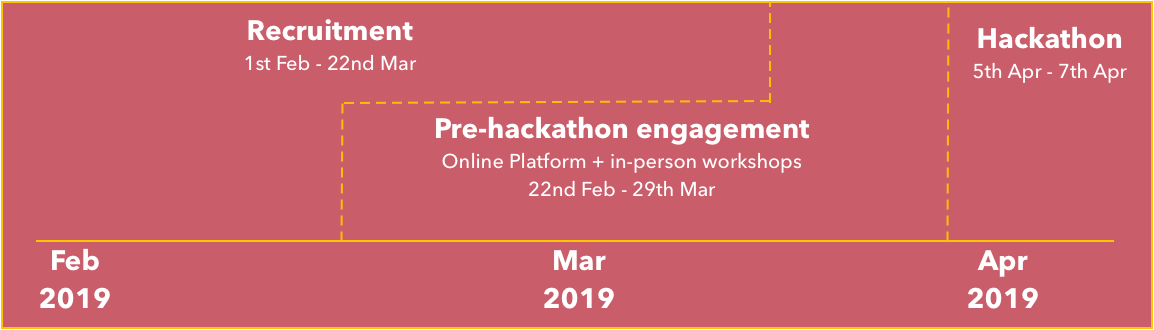
\includegraphics[width=.8\linewidth]{Images/DemVR/Timeline.jpg}
\caption{Timeline of the event}
\label{fig:DemVRTimeline}
\end{figure}

In 2019, I set out to organise a hackathon called DemVR, both to generate a set of bespoke VR environments for those living with dementia, as well as to consider how developers/designers (with expertise in media or VR) and people living with dementia may collaborate. Inspired by prior work involving lived experiences in hackathons \citep{birbeck_self_2017}, the hackathon was split into two engagement phases see Fig.\ref{fig:DemVRTimeline}. The first was a six-week pre-hackathon phase: this consisted of the deployment of an online platform (called Ideaboard) to support designers/developers in pitching their potential hackathon ideas and receiving feedback from people living with dementia and care partners. The second phase was the two-day hackathon event itself, where participants formed teams to compete for £1,000 \& £500 prizes by creating prototypes of VR experiences for people living with dementia and their care partners. To accommodate funding for venue hire, branding, food and travel, I partnered up with several organisations in Newcastle who assisted in the funding and providing expert knowledge on dementia, VR, and running tech-focused events. For instance, continuing my relationship with Silvelrine Memories provided the hackathon with dementia expertise, while connecting with Sunderland Software City provided funding for venue hire. In the following sub-sections, we describe the event according to the timeline of the hackathon: a) recruitment; b) pre-hackathon - online platform, in-person workshops, team formation event; and c) the two-day hackathon.

\subsection{Recruitment}
\label{sec:EventRecruitment}
My initial recruitment process targeted designers and developers through university networks, VR/AR labs across the UK, as well as publishing blog pieces on popular VR websites to invite creators to take part in the two-day event. Upon registering for the event on our website\footnote{www.demvr.uk}, participants were sent an email inviting them to sign up for Ideaboard and submit their idea, I attempted to recruit people living with dementia and their care partners in multiple ways. The first, was through Silverline Memories who I talk in detail about in chapter \ref{NegotatingReseacherParticipantRelationships}. Secondly, given Twitter is a popular social media platform for dementia network and advocates \citep{talbot_how_2020}, I ran a Twitter account posting tweets to encourage people living with dementia and their care partners to sign-up. In these instances, while I invited people with dementia and care partners to the hackathon, the priority was signing them up to the online platform or take part in the in-person workshops as the pre-engagement phase supported longer-term engagement. However, as I mentioned in this chapter, our recruitment process to involve people living with dementia and care partners failed with only one care partner signing up to our platform.

Within our hackathon participant recruitment, the majority of attendees had to some degree experience with technical, design and/or research skills. While we did invite care partners, social workers and practitioners, the high-level expectation of building demos or lo-fi prototypes for virtual reality experiences could have intimidated those with less technical backgrounds from participating resulting in a \textit{“limiting difference among participants” }\citep{irani_hackathons_2015}. Additionally, the technology-oriented event may have contributed to the lack of interest from people with dementia and care partners. For instance, \cite{hwang2020exploring} recommend researchers should provide a longer-term learning and facilitating process with people with dementia to promote inclusion and learnability. While we discuss meeting people with dementia where they are in detail in our discussion as a reflection on our lack of engagement through online platforms, appropriation of hackathon knowledge including insights into VR in the recruitment stage could have been more carefully considered. Furthermore, the authors highlight if the learning process for engagement evokes \textit{“frustration, anxiety, or sense of vulnerability (pg.46:26)\citep{hwang2020exploring}}, then the person with dementia may resist the interest or engagement with that particular technology. Despite our efforts to invite people with dementia from our partner charity who had previous interests and knowledge into VR from prior studies seen in \ref{NegotatingReseacherParticipantRelationships}, neglecting a set of resources for the recruitment stage to upskill people with dementia, care partners and the public onto the topic of designing VR experiences likely contributed to an unawareness or confidence to share experiences online and during the two-day event. We return to these challenges in our discussion.

Twelve participants (2 women, 10 men) actively signed up to the online platform. During set up, to get the conversation rolling, I added three initial example ideas focused on shared family VR environments, personalising the VR headset, and a VR experience that blends the real world and virtual into one. Out of the twelve participants, eight submitted ideas. Of the twelve participants, nine attended the hackathon (see table \ref{table:DemVRDemographic}), with two of them submitting an idea but not attending the hackathon. One participant, a care partner named Denis, was unable to attend the hackathon but actively joined discussions on six of the submitted ideas. Additionally, while we set-up two in-person workshops described in \ref{sec:EventPrehackathon}, the workshops received no sign-ups resulting in no additional feedback for teams from people living with dementia or their care partners. In the following sections, I dive into this further considering why this may have been the case. 

For the hackathon, I had 40 participants (18 women, 22 men) attend. In our pre-hackathon team formation stage, I had an additional team of four that dropped out due to intellectual property concerns. This resulted in nine teams. Individual demographics of participants within their associated teams are summarised in table \ref{table:DemVRDemographic}. Although no participants had the experience of being a care partner or living with dementia, participants identified their experience with dementia during the sign-up process from the following: 

\begin{itemize}
\item{\textbf{Experienced}: worked in the area of dementia in a research/industry/care setting/charity.}
\item{\textbf{Knowledgeable}: Has had a family member or friend living with dementia but not necessarily cared for them.}
\item{\textbf{Limited}: Have read people's experiences or recent research in the area of dementia.}
\item{\textbf{None}: Know very little about the topic}
\end{itemize}

% custom commands
\newcolumntype{L}[1]{>{\raggedright\let\newline\\\arraybackslash\hspace{0pt}}p{#1}}
\newcolumntype{C}[1]{>{\centering\let\newline\\\arraybackslash\hspace{0pt}}p{#1}}
\newcolumntype{R}[1]{>{\raggedleft\let\newline\\\arraybackslash\hspace{0pt}}p{#1}}

% this line fixes the vertical padding of text inside the cells
\renewcommand{\arraystretch}{1.4}

\begin{table*}[htp]
\begin{tabularx}{\textwidth}{@{} YYYYYY @{}}
\hline
\textbf{Team} & \textbf{No. members} & \textbf{Age range} & \textbf{Background} & \textbf{Experience with dementia} & \textbf{No. Ideaboard\footnote{members who joined Ideaboard}} \\ \hline 
Garden Life & 7 & 16-25 & Comp-sci undergrads (7) & Limited (1) / None (6) & 3 \\ \hline
Chatter Bench & 2 & 26-45 & History researcher (1) / HCI research developer   (1) & Experienced (1) / Limited (1) & 0 \\ \hline
Augmented World & 6 & 16-25 & Comp-sci undergrads (6) & Limited (2) / None (4) & 1 \\ \hline
VRHallucinate & 6 & 16-35 & Psychology researcher (2) / Developer (3) /   Designers (1) & Limited (1) / None (5) & 0 \\ \hline
LookingVRBack & 4 & 25-45 & Marketing (1) / Biomedical researcher (1) /   Comp-sci undergrad (2) & Experienced (1) / None (3) & 2 \\ \hline
Mindful Forest & 2 & 16-25 & Comp-sci undergrad (2) & Passing (2) & 0 \\ \hline
Sensory Tide & 6 & 26-45 & HCI researcher (3) / Developer (1) / Filmmaker   (2) & Experienced (2) / Passing (1) / None (2) & 3 \\ \hline
World Share & 3 & 16-25 & Filmmaker (3) & Passing (1) / None (2) & 0 \\ \hline
VRmotion & 4 & 16-25 & HCI researcher (1) / Developer (1) / Designer   (2) & Experienced (1) / Limited (1) / None (2) & 0 \\ \hline
\end{tabularx}
\caption{DemVR participant table}
\label{table:DemVRDemographic}
\end{table*}

Expert speakers were also invited to discuss topics on design, dementia advocacy, and experiences of living with dementia. An additional three dementia \& HCI researchers, a gerontologist, and the CEO of Silverline Memories, assisted with hackathon facilitation. The facilitators' role lent their experience by sitting down with individual teams throughout the two days to talk through the teams' ideas and thought processes. Our judges consisted of a dementia HCI research, the CEO of Silverline Memories, a VR expert, and an accessibility HCI researcher to judge the team's final VR ideas.

\subsection{Pre-hackathon engagement}
\label{sec:EventPrehackathon}
I planned and arranged a six-week consultation period, to be carried out via 1) an online participatory platform, and 2) in-person workshops with people living with dementia, and their care partners. Additionally, I provided a team formation day prior the two-day hackathon to ensure participants. The pre-hackathon stage provided the optional opportunity for future hackathon participants to submit initial thoughts and ideas where experts would provide feedback to give participants insight into the wants, desires, and experiences of people with dementia and their care partners. 

\subsubsection{Online platform (Ideaboard)}
\label{sec:Ideaboard}
The participatory platform, Ideaboard\footnote{www.Ideaboard.co.uk}, was conceptually developed in-house at Open Lab from prior participatory platforms in working in Digital Civics and social care - for instance, one inspiration was App Movement \citep{garbett_app_2016}, a platform that enables users to \textit{"collaborate, design, and deploy community commissioned mobile applications"}. Ideaboard similarly offers creative tools and workspaces to support the creation of ideas and collaboration. Here I describe the process users undertake to add ideas to the platform. Our Ideaboard process was split into three components:

\begin{enumerate}
    \item On Ideaboard, participants were invited to share preliminary ideas that they could develop during the in-person hackathon. Once their idea was uploaded, participants could then explore and comment on other submitted ideas (see Fig.\ref{fig:exploreIdeaboard}).
    \item Once participants had submitted their ideas, we invited people with dementia and their care partners to share insights and critique the submitted ideas before the hackathon through an open forum. We hoped that this would allow people who might be unavailable for the hackathon to take part in design ideation and help to shape emerging ideas which might be taken further in the in-person sessions. 
    \item Hackathon participants could then respond to the expert feedback and begin an open dialogue with other participants, care partners and people with dementia. From here, teams have more in-depth and developed ideas that consider the experiences of care partners and/or people with dementia that they could continue to develop and ideate on throughout the two-day hackathon. 
\end{enumerate}

\begin{figure}
\centering
\begin{subfigure}{.5\textwidth}
  \centering
  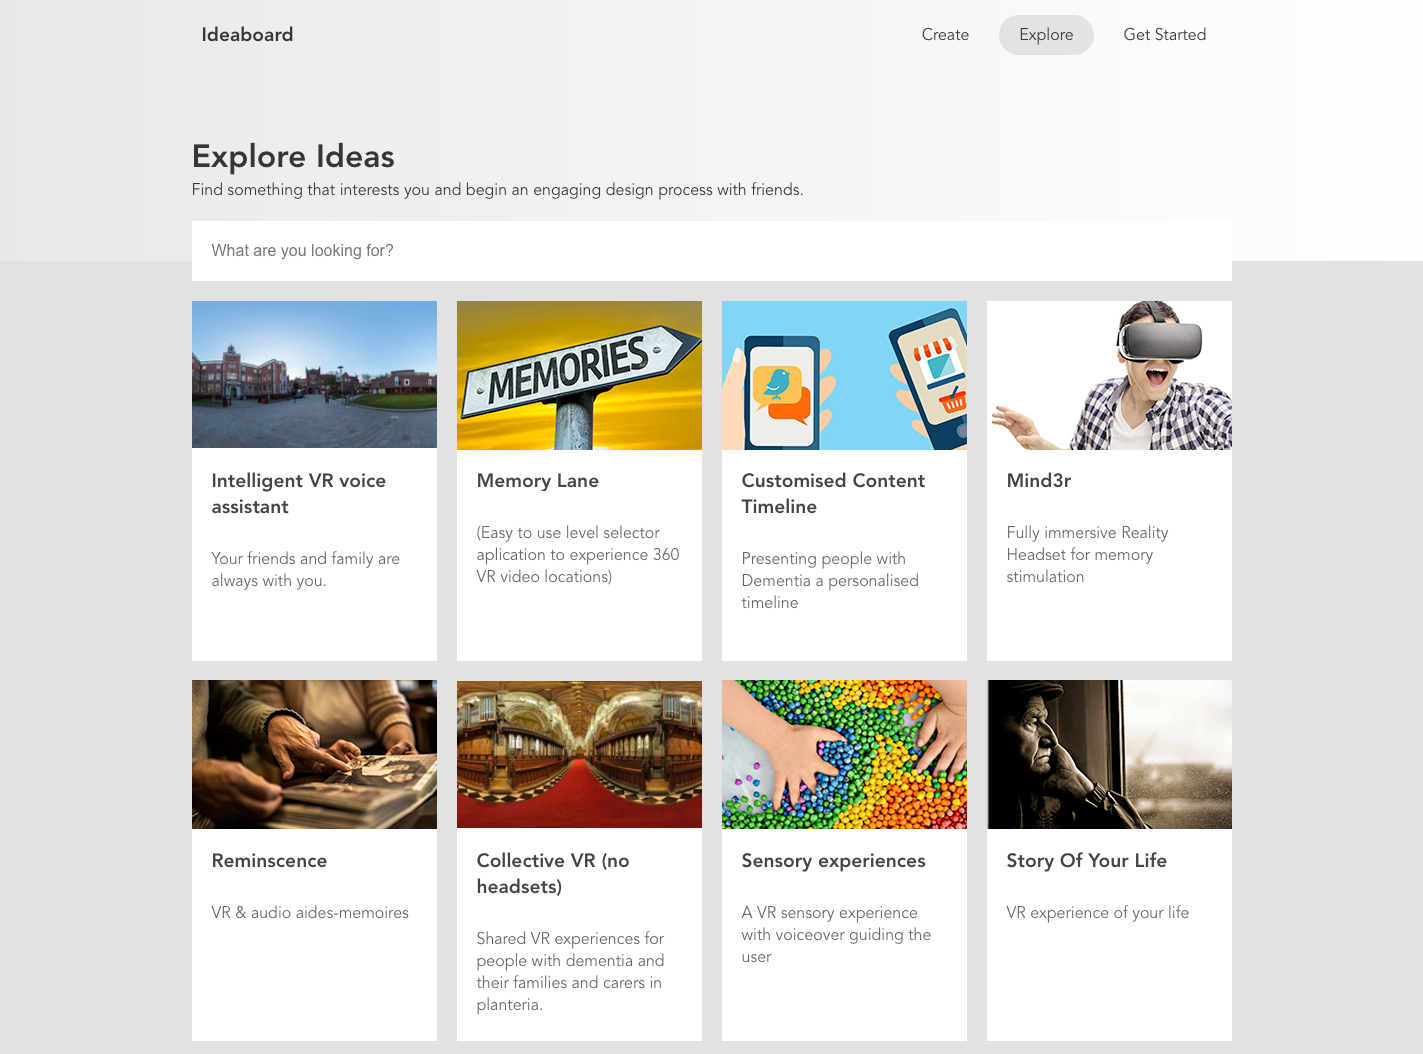
\includegraphics[width=.8\linewidth]{Images/DemVR/Ideaboard Ideas.png}
  \caption{Explore Ideaboard ideas}
  \label{fig:exploreIdeaboard}
\end{subfigure}%
\begin{subfigure}{.5\textwidth}
  \centering
  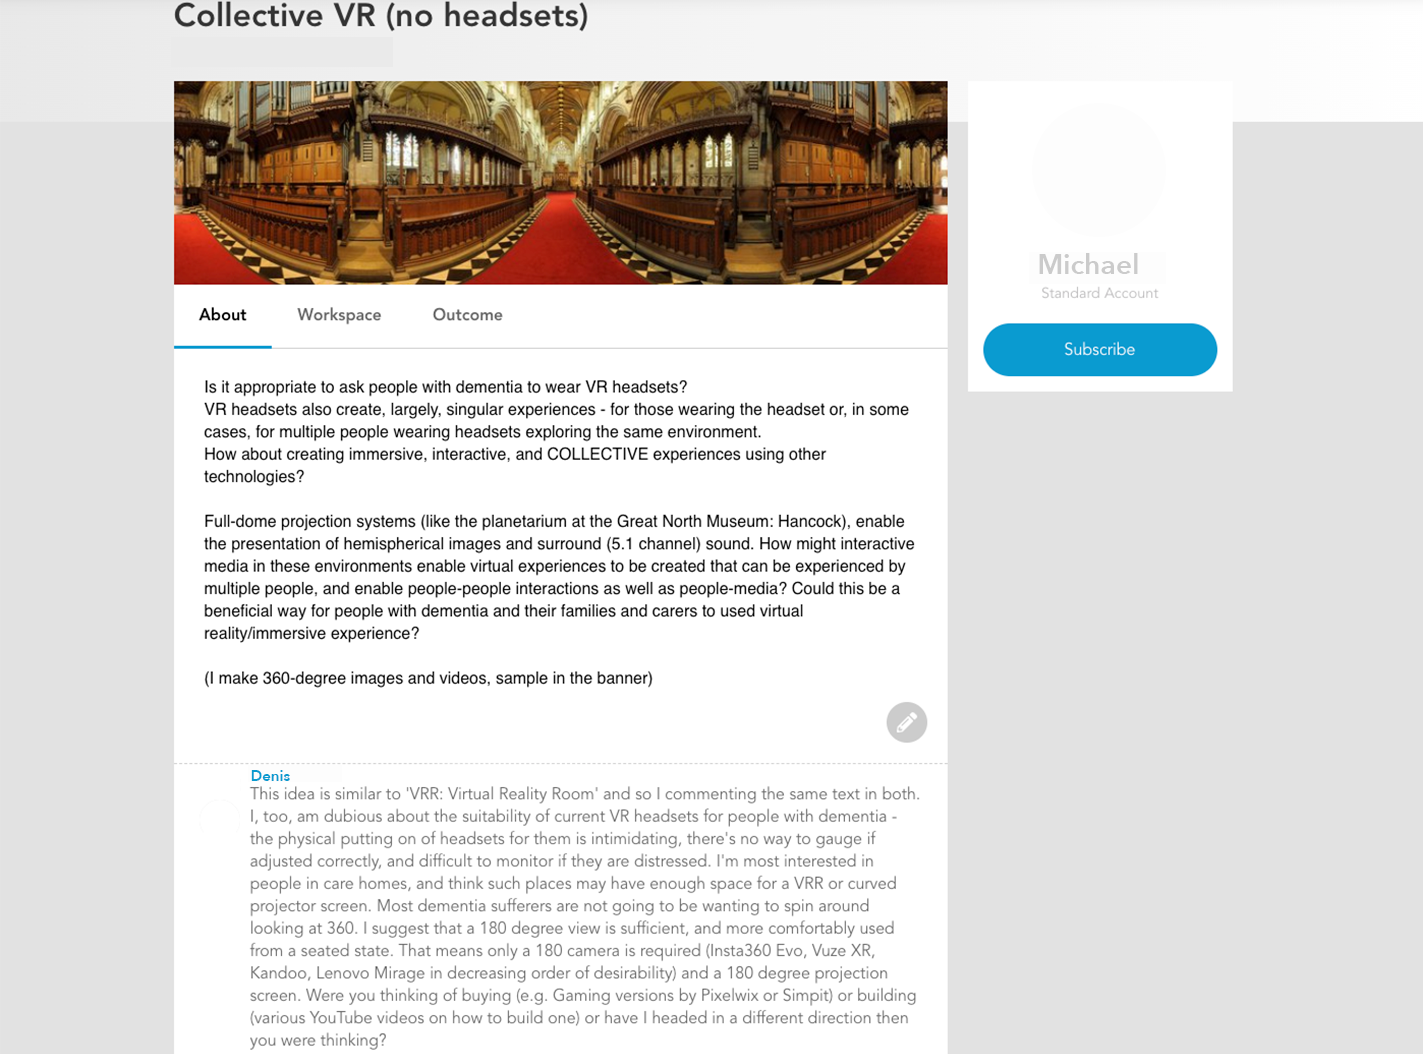
\includegraphics[width=.8\linewidth]{Images/DemVR/Example of idea.png}
  \caption{Example of 'idea' features}
  \label{fig:IdeaboardIdea}
\end{subfigure}
\caption{Ideaboard features}
\label{fig:IdeaboardFeatures}
\end{figure}

\subsubsection{In-person workshops}
\label{sec:in-personWorkshops}

To further support participation beyond the online platform \citep{piper2016technological}, I set up two in-person workshop sessions inviting members of a local dementia café. Working closely with the dementia café on prior VR projects, I expected to recruit several people with dementia and care partners with established experience of VR. Within the six-week consultation period, the two in-person workshops were organised in the final two-weeks to ensure the I could print off any submitted Ideaboard ideas to share with participants.  This workshop was intended to support participants to engage in a set of design activities to illustrate their desired VR shared experiences or build upon the existing eleven ideas posted on Ideaboard. Based on comments and ideas produced in these workshops by care partners and people with dementia, I would then add any additional ideas to Ideaboard or add any comments made about existing ideas to the relevant Ideaboard idea. I hoped that this process would allow the designers/developers to have additional time to reflect on comments from people with dementia and their care partners. As stated in the recruitment, the attempts to involve people with dementia and their care partners was significantly limited to one care partner’s involvement which engaged through the online platform. For both in-person workshops, we had no sign-ups meaning we had to cancel the workshops. I refer to this in more detail through the findings and discussion.

\subsection{Team formation}
\label{sec:TeamFormation}
I also set up a 2-hour pre-hackathon team formation event on the Friday of the hackathon event to ensure participants had organised themselves into teams. During the team formation event, I printed the eleven ideas published on Ideaboard. O placed them on individual tables with sticky notes to express an interest in the idea or find other participants who may also be interested in developing the ideas further. Since submitting an idea on Ideaboard was optional, five teams came prepared with ideas. As a result, only four of the eleven Ideaboard posts were taken into the hackathon. In table 3, I present the origin point of teams’ initial ideas. While only four Ideaboard posts were adapted and built upon through the hackathon, the other five teams’ either came with a bespoke idea they kept to themselves or proposed an idea at the start of day one. During the hackathon, all teams adapted their original ideas by reflecting on dementia through a series of resources (that I discuss below) and used the time to build and design a technical prototype of their VR experience. 

\subsection{Hackathon}

\begin{figure}[htp]
\centering
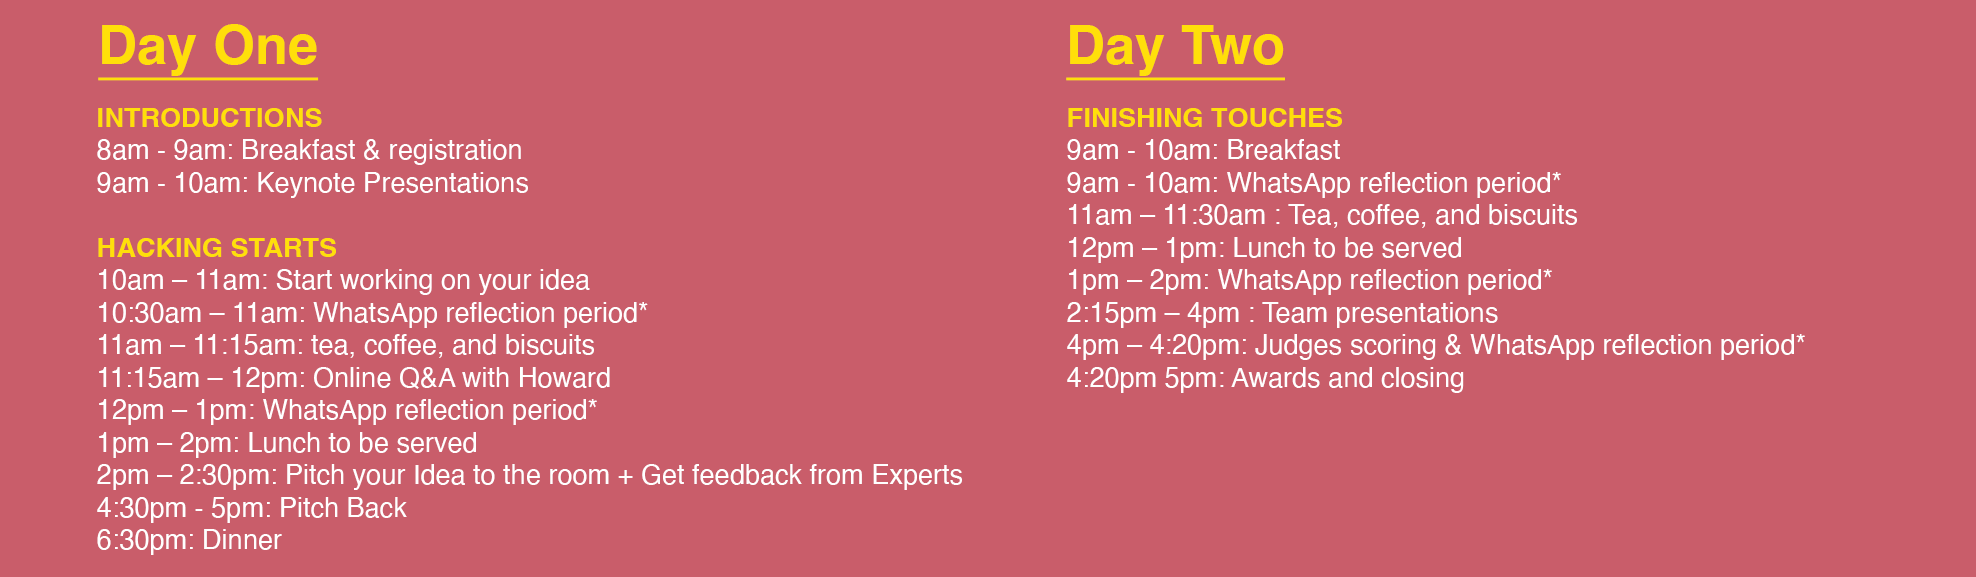
\includegraphics[width=1\linewidth]{Images/DemVR/DemVRHackathonSchedule.png}
\caption{DemVR hackathon event schedule}
\label{fig:schedule}
\end{figure}
The hackathon too place across one weekend (April 5\textsuperscript{th} - 7\textsuperscript{th} 2019), at a local museum in Newcastle. The venue is centred within the city centre near the University campus and co-exists alongside a Natural History Museum that attendees had access to throughout the two-days that provided space away from ‘hacking’. To accompany the large number of teams and space required for VR demos, each team received a demo space, rounded table, and an array of crafting materials. For additional details of the schedule, check out our online appendix. In terms of equipment, teams had access to eight Oculus Go’s, four Oculus Rifts, one HTC Vive, and two VR-ready PC rigs. Teams were encouraged to bring their laptops and VR kit if they wished, and to notify the facilitators before the event if they need any additional technologies.

To encourage participants to ask for expertise feedback or general queries, each team were provided with a WhatsApp group consisting of 1-2 facilitators who could respond over text, or to be asked to join the team in person. In practice, these online chats provided quick and easy links to papers or method approaches that were related to the topic at hand. Furthermore, we used these groups chats as an opportunity to a) ask participants to respond to reflective questions such as "how have your thoughts about dementia and/or virtual reality changed from the beginning of day one?" and “describe your reaction to Howard’s Q\&A”, and b) to see the teams’ design processes throughout the two days. For instance, team Sensory Tide shared several pictures of team members traveling to a local beach to collect videos and shells to be used in their finalised idea. 

\subsubsection{Day One}
\label{DayOne}

\begin{figure}[htp]
\centering
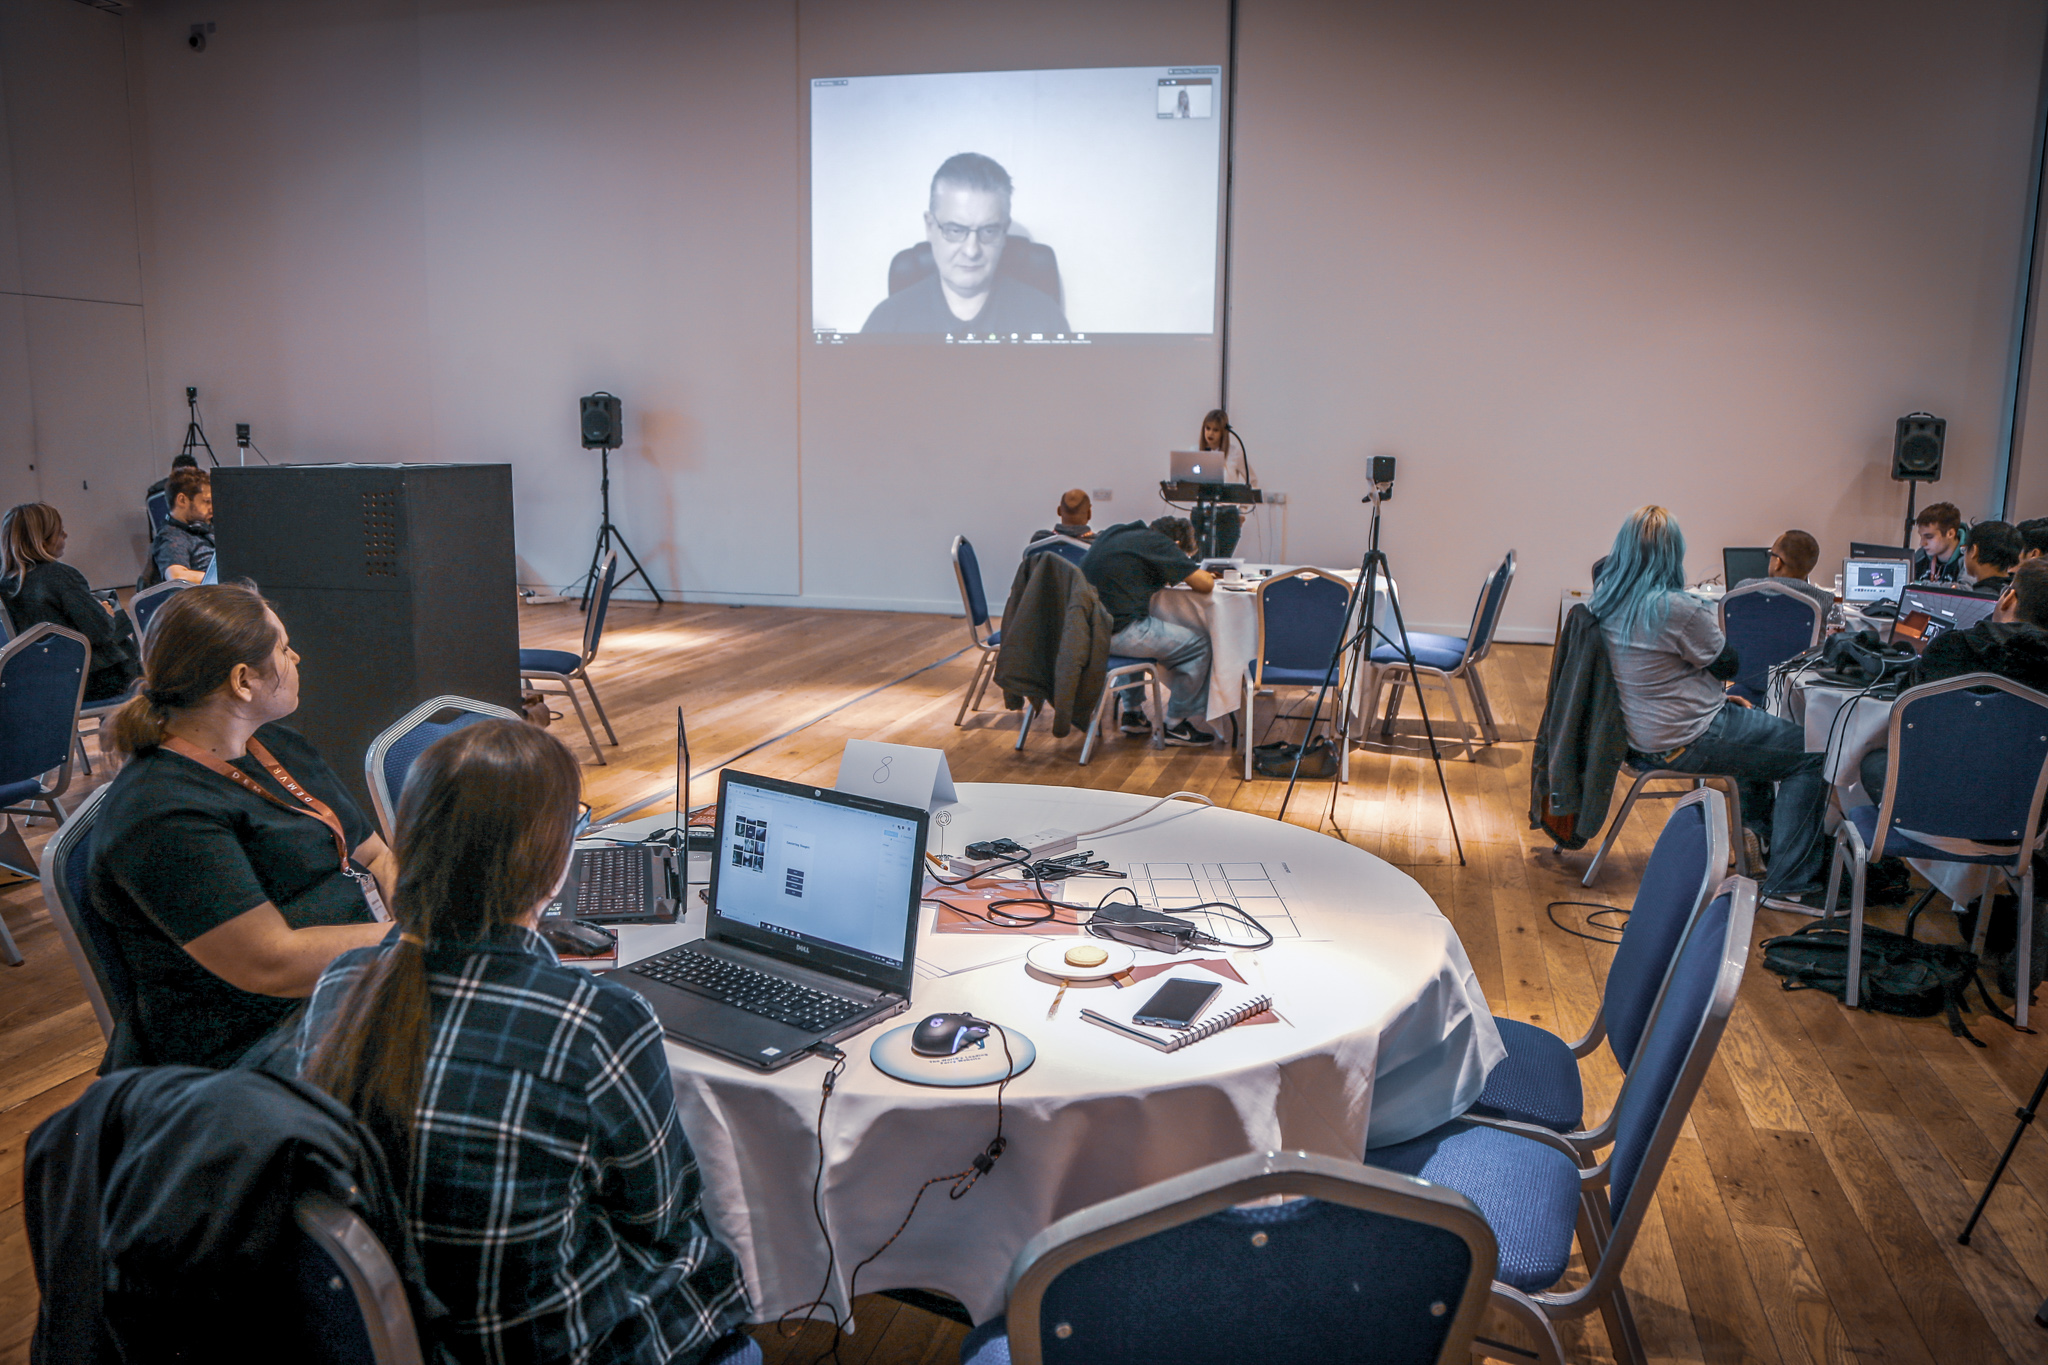
\includegraphics[width=.8\linewidth]{Images/DemVR/Howard.jpg}
\caption{Howard's Zoom Q\&A}
\label{fig:Howard}
\end{figure}
The first morning of the event consisted of presentations on dementia, participatory research, and virtual reality by invited speakers. The invited speakers also enacted as facilitators that provided hackathon participants insight into the several facilitators backgrounds. During mid-day, we organised an online Q\&A with Howard, a dementia advocate who shared his experiences living with dementia that lasted 15 minutes. In the Q\&A, Howard was asked about his challenges of being diagnosed, the type of technologies and experiences he would find useful, and the social complexities he is currently facing given the stigma of dementia. While the Q\&A was open for questions from the participants, the conversation was led by one of the keynote facilitators who has a strong relationship with Howard (see fig.\ref{fig:Howard}. 

Teams could then ask for additional help or critique from the available facilitators via in-person or reaching out to the facilitators in the individually set up WhatsApp team groups. In practice, these online chats with facilitators provided quick and easy links to papers or method approaches that were related to the topic at hand. Furthermore, we used these groups chats as an opportunity to a) ask participants to respond to reflective questions such as "how have your thoughts about dementia and/or virtual reality changed from the beginning of day one?" and “describe your reaction to Howard’s Q\&A”, and b) invited to detail their project’s progression through submitting comments, audio recordings and videos through a dedicated Team WhatsApp group chat, which formed the basis of data collected during the event. For instance, team Sensory Tide shared several pictures of team members traveling to a local beach to collect videos and shells to be used in their finalised idea.

Teams were given inspiration packs (see figure \ref{fig:InspirationPacks}): these consisted of materials that summarized key insights from previously published work on VR and dementia from \citep{hodge_exploring_2018}. In addition to the physical inspiration packs, we set up an online shared document that would continue to grow as a resource through the duration of the event. In the end, this consisted of academic papers; speaker slides; dementia guides such as DEEP language and NHS (UK National Health Service) guides; a set of design method processes such as scenarios, bodystorming, and 5 Whys; and tips and tricks for what to include in final presentations. In our findings, the DEEP language guide is drawn on several times and is worth describing further. The DEEP language guide is a three-page document designed by 20 people living with dementia. The key takeaways of the document are a set of standards for dementia terms such as 'with' or living well' with dementia. During the afternoon, all teams pitched their idea to the rest of the room that provided an open forum between facilitators and participants to provide additional feedback for the set of ideas. For the rest of the weekend, the teams worked on their ideas with periods built in for breaks and socialisation. 


\begin{figure}
\centering
\begin{subfigure}{.5\textwidth}
  \centering
  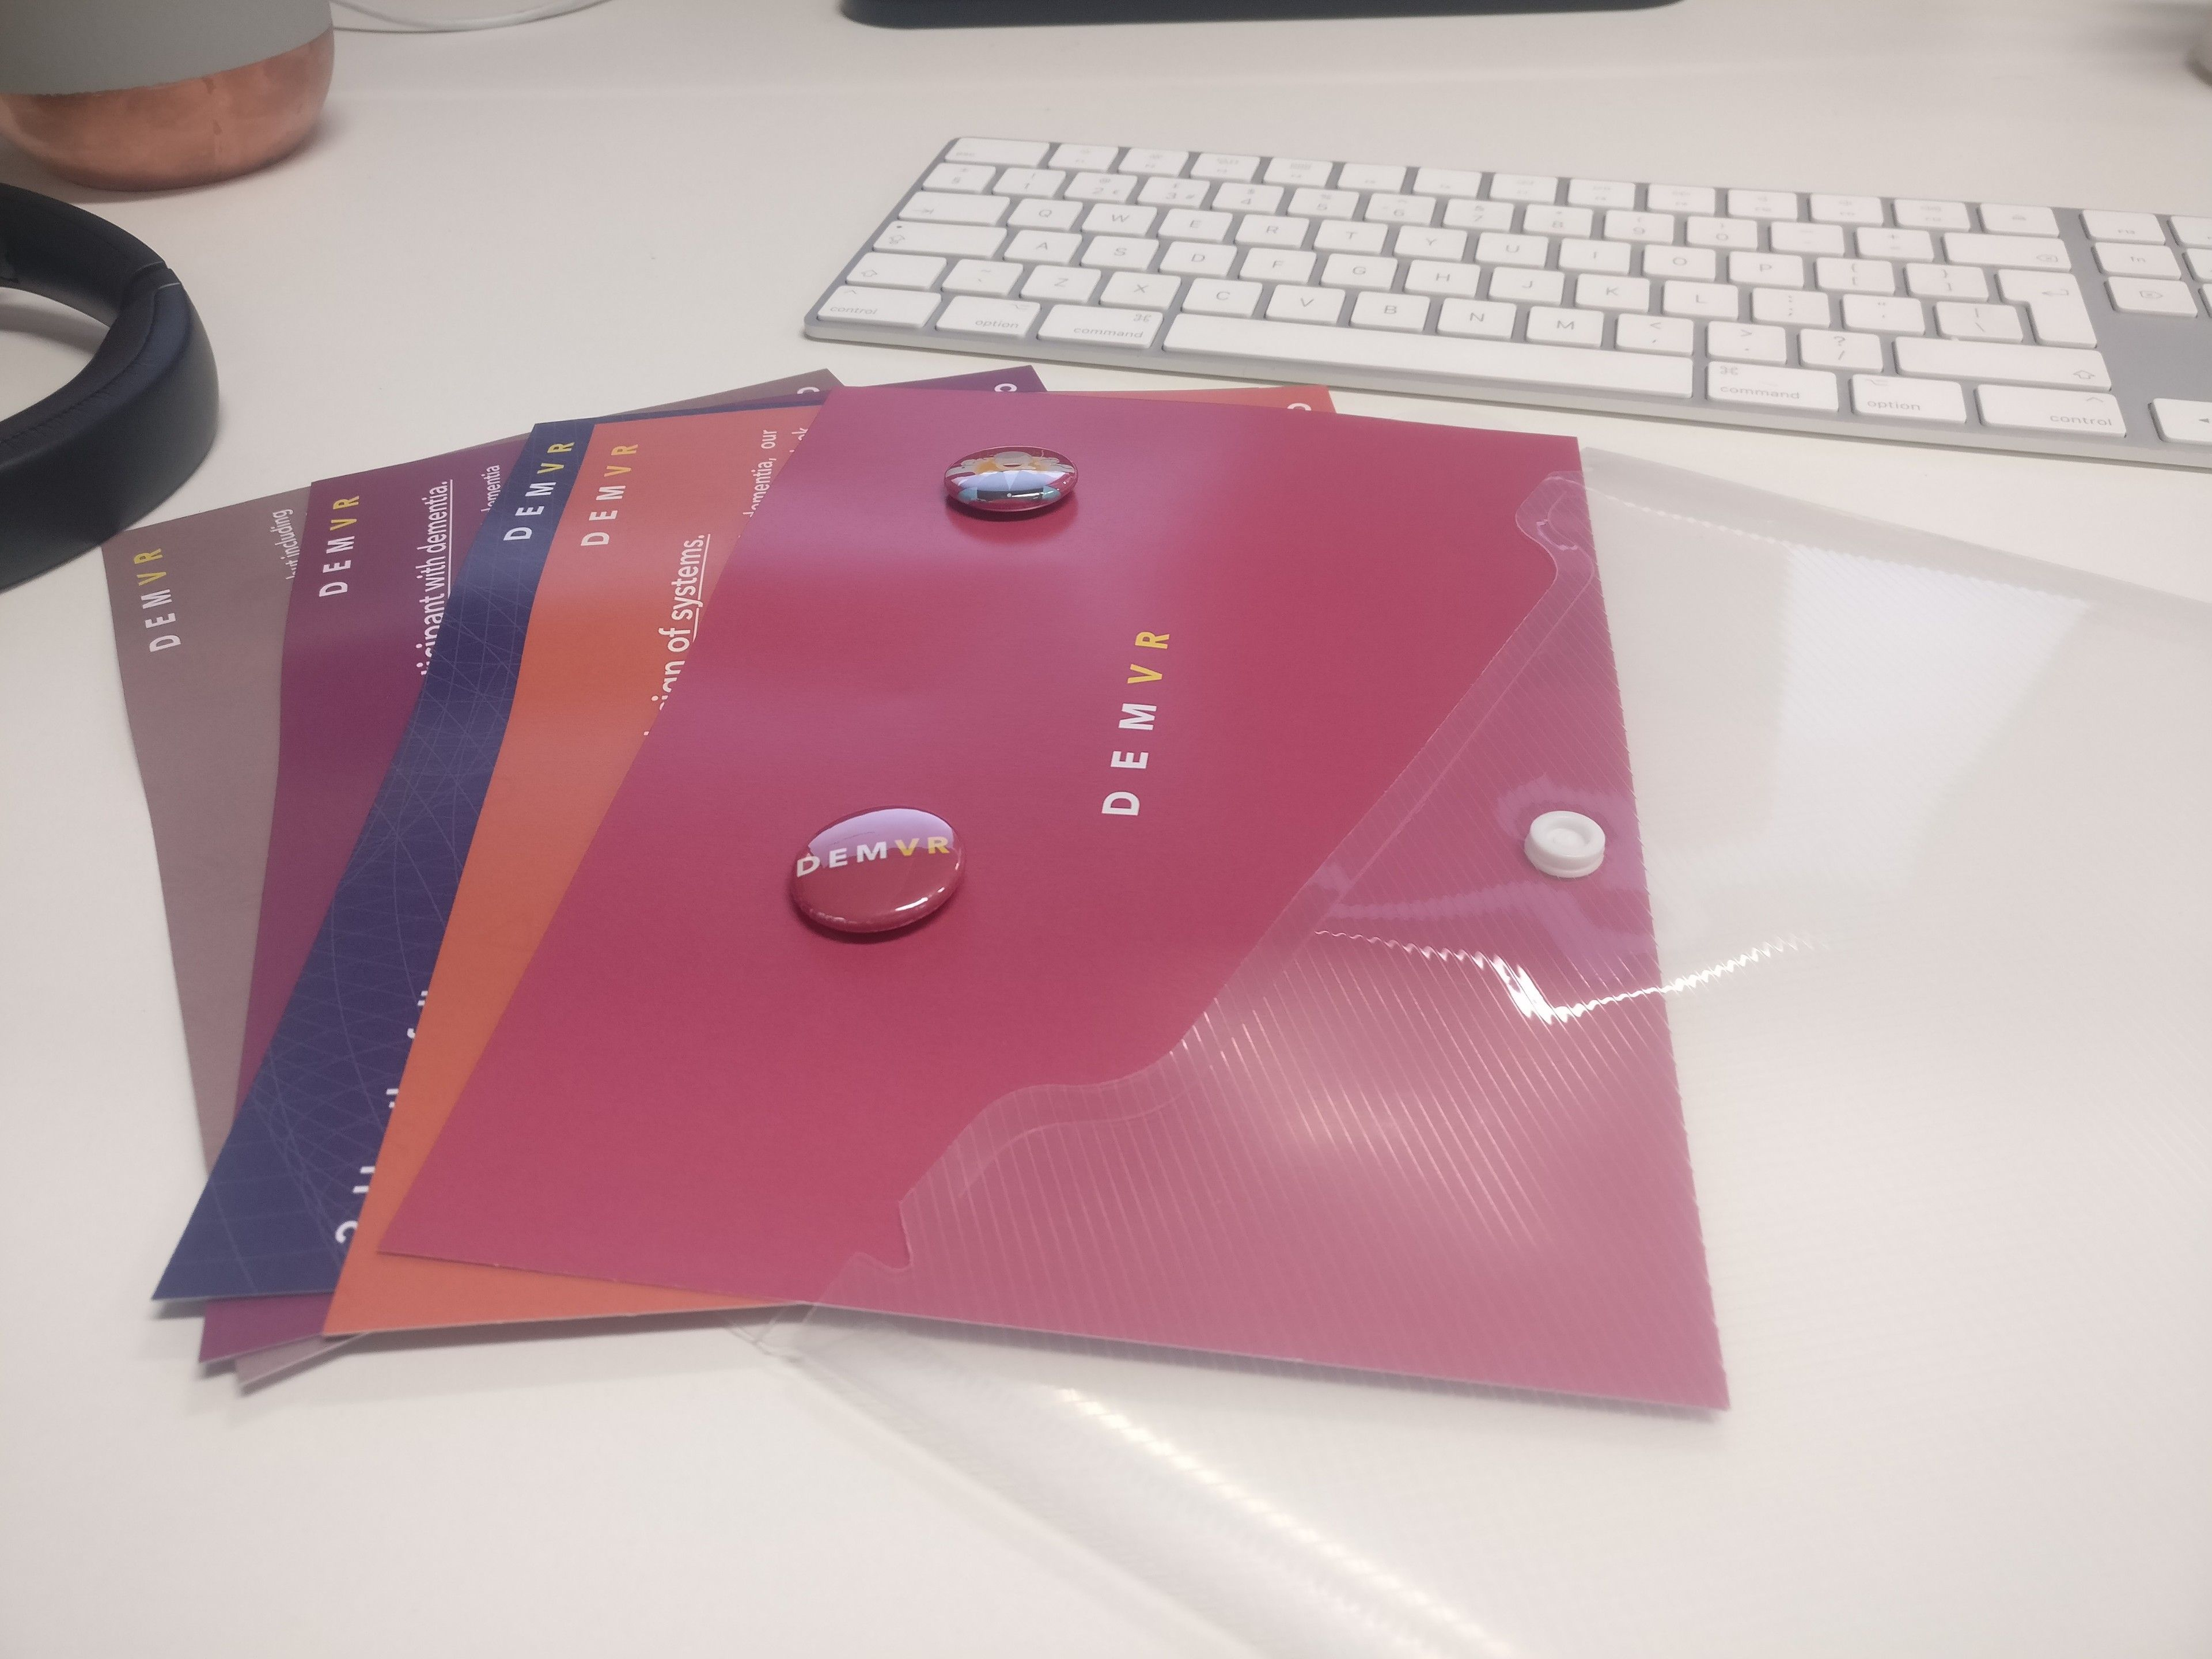
\includegraphics[width=.8\linewidth]{Images/DemVR/DemVRInspiration.jpeg}
  \label{fig:InspirationPackImage}
\end{subfigure}%
\begin{subfigure}{.5\textwidth}
  \centering
  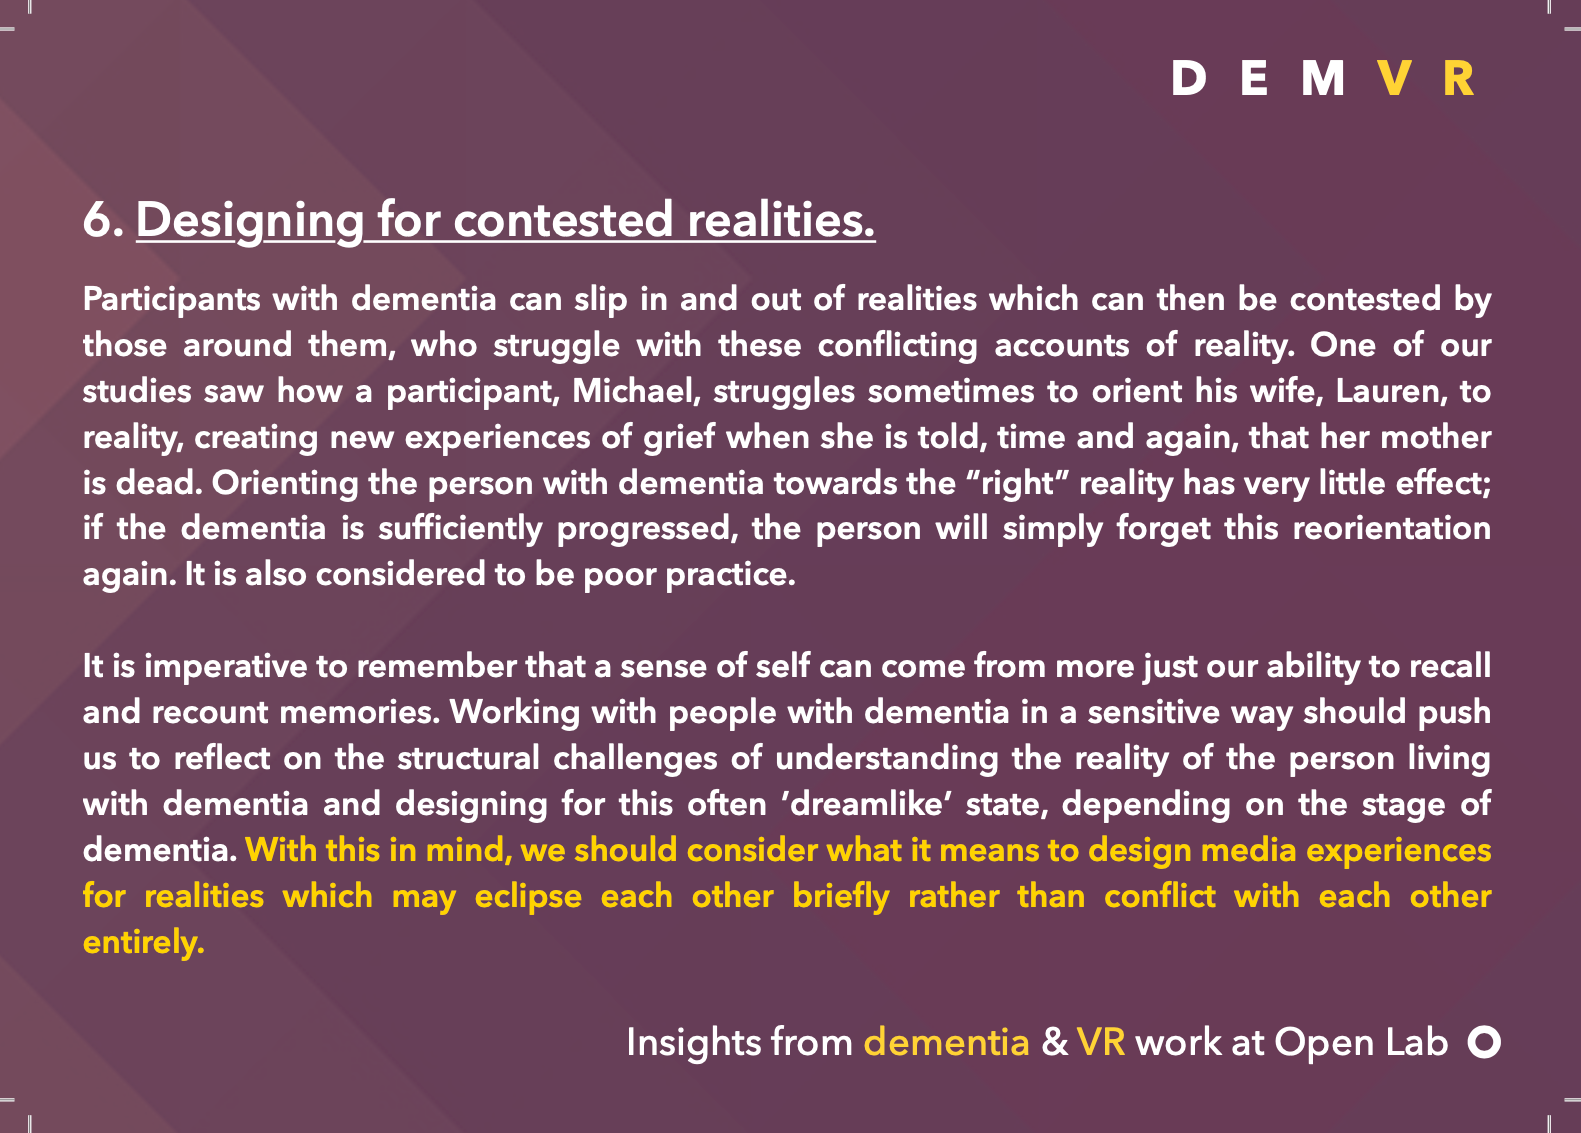
\includegraphics[width=.8\linewidth]{Images/DemVR/InspirationCard.png}
  \label{fig:InspirationCard}
\end{subfigure}
\caption{Inspiration packs}
\label{fig:InspirationPacks}
\end{figure}

\subsubsection{Day Two}
\label{DayTwo}
On the Sunday morning, teams had the entirety of the day to finalise their ideas and presentations and have opportunity to ask facilitators for any feedback on their presentations and demo. For the majority, facilitators assisted in helping the teams add finishing touches to their demo’s and providing feedback for their presentations. To maintain consistency throughout the team presentations, we provided a template with conversation topics such as: tagline; who is your user audience; what is your motivation and problem; what was your approach to inform your design challenge; what are the future considerations; and reflection on the hackathon. The event culminated in a final ten-minute presentation and five-minute demo at the end of day two in which the teams demonstrated their work to the judges. The four judges had the opportunity to explore the demo along with ask any further questions about the teams finalised idea. Each team’s finalised concepts were rated on the following:
\begin{itemize}
\item novelty of design concept: how original are the ideas? Are they backed up with appropriate research? How provocative (yet sensitive) or otherwise promising are they?
\item clarity of team's vision: How persuasive are the presented arguments?
\item sensitivity to the challenge: Specificity to issues central to dementia/care; how well were experts’ suggestions taken on board; are there any potential negative consequences?
\item potential for real-world impact: given appropriate backing or resource, would this concept make a difference?
\item strength of VR/AR: How far along did the idea development get? Did the teams make good use of the technology at hand? 
\end{itemize}

At the end of the day, the judges announced the 1st and 2nd place winners who would receive £1000 and £500, and the event ended with a brief overview of the hackathon by the first author. 



\section{Methodology}
\label{sec:methodology}
In the following section, we describe our positionality, ethics, data collection and analysis process and provide a summarized table of the proposed vs. final team ideas.

\subsection{Positionality}
\label{method:positionality}
Following the event, I began to process and reflect on how the event went and what the contribution was to HCI research. From early on, it was apparent that while the nine teams had created bespoke shared VR experienced prototypes, I felt that the lack of involvement of people living with dementia was significantly reflected in teams' presentations, raising concerns as to how designers/developers may design for dementia without these lived experiences front and centre in their design processes. Given this, it is worth writing that my positionality as a dementia researcher was an integral influence in the hackathon's facilitation and subsequent evaluation of the event \citep{bourke_positionality_2014}. During the study's framing and running of the event, I selected particular researchers who take a similar approach to dementia through using a person-centered design approach. While this was intentional as I wanted to explore ways to scale person-centered approaches, the orientation towards how I view dementia influenced the hackathon's framing by emphasising participants to take a more creative and well-being approach to their design instead of problematising someone's cognitive deficits. Furthermore, I hand-picked the facilitators who also take a more relationship and meaningful interaction to their work instead that of a biomedical one. By carefully selecting particular facilitators and presenters, it is likely that this impacted the teams' final prototypes and potentially limited the potential of teams to develop more biomedical led design approaches. 

Given the clear challenges I faced in representation of people with dementia and their care partners, I saw this as an opportunity to provide guidance for future researchers on the potential knock-on effects that may occur when designing for a group or person are overlooked. Motivated by the questions posed by the literature mentioned above and our internal reflections on the facilitating and developing of our hackathon event, I present the following research questions, which guided our analysis:

\begin{itemize}
    \item \textbf{Research Question One:} What type of motivations and ‘on-site’ learning may occur when learning about dementia within a hackathon setting?
    \item \textbf{Research Question Two:} What design approaches do designers and developers prioritise when designing for people with dementia?
    \item \textbf{Research Question Three:}What challenges may arise when shaping a VR experience for people with dementia and care partners when solely relying on the designer/developer’s own experience (or lack thereof)?
\end{itemize}

\subsection{Ethics}
\label{sec:Ethics}
Ethical approval was granted by Newcastle University. Upon signing up, each participant was provided with an information and consent form describing the event and pre-hackathon stage. Any participants who then signed up to use our online platform was given additional information about the project. Participants who registered for the hackathon signed a consent form about the hackathon weekend when they came to pick up their lanyard and sign in for the opening day of the hackathon. Participants’ and team names have been anonymised for privacy.

\subsection{Data and Analysis}
\label{sec:DataAnalysis}
In the study, I gathered data from three different source: 1) Text data of the Ideaboard ideas (I), including additional comments from participants on the ideas; 2) Keynote, Q\&A and teams’ presentations from the event (P) and; 3) Each team WhatsApp group’s text, images and audio, which were extracted using the built-in Google Drive feature. WhatsApp audio recordings were also transcribed and anonymised by UKTranscription (W). To provide an additional context, I made a set of observational field notes (F) throughout the event highlighting conversations I had with teams and facilitators. The initials (I, P, W, or F) indicate the source of the data in the findings.

\begin{table*}[ht]
\caption{}
\label{table:data collection}
\begin{tabularx}{\textwidth}{@{} Y|YYYYY @{}}
\textbf{Stakeholders} & \textbf{Ideaboard (I)} & \textbf{WhatsApp (W)} & \textbf{Presentations (P)} & \textbf{Field notes (F)} \\ \hline
Hackathon participants & 11 submitted ideas & 25 minutes audio recordings + average 25 texts per team & 117 minutes & N/A \\
People with dementia and care partners & One care partner replied to eight submitted ideas & N/A & 15 minutes Q\&A & N/A \\
Facilitators & N/A & Average 6 texts replying to each team & 40 minutes & 11,355 words \\
\end{tabularx}
\caption{Data collection}
\end{table*}
My analytic approach followed a Thematic Analysis (TA) set out by \cite{braun_one_2020,braun_using_2006}. Working from multiple data sources, I ordered the individual sets of data across a timeline to make sense of interactions between data sets. This approach helped to decide if it was possible that a certain event, such as a keynote or the Q\&A, had influenced a team's design approach, though our qualitative approach is careful in not claiming causality. Second, the I structured a set of team narratives consisting of the different data sources described above. Structuring the data this way helped to describe the chronological development of each individuals’ teams from design ideation through to presenting their final idea and post-hackathon reflections.  Once the data was framed chronologically, I began to conduct open coding. I then meet bi-weekly with Dr Kellie Morrissey, Dr Sarah Foley, and Dr Dave Kirk to construct themes and reflect on the patterns evident across the data. Finally, the I constructed the named themes, which are presented in the following section. 

\section{Findings}
\label{sec:Findings}
This section presents a series of findings that centre around two overarching themes describing insights into participants interactions and design considerations through the event. The first theme examines participants' approaches to engagement and design: this explores their motivations for taking part in the event, as well as analysing how participants attempted to incorporate their new understandings of dementia into their design. The second theme, reworking participants’ conceptualizations for design, describes the challenges of assimilating these sensitivities into design outcomes, given the absence of crucial stakeholders.

\subsection{Participants' approaches to engagement and design}
\label{LearningEvent:ThemeOne}
As mentioned in our literature review, participation in design events is significantly labour-intensive and time-consuming, yet they remain a popular route for learning and developing new paths to research. Further, hackathons provide attendees an opportunity to learn new soft skills and new insights into areas they may have yet explored \citep{medina_angarita_what_2020}. The following subthemes describe what motivated participants to spend their weekend ‘hacking’ away and how incremental, ‘on-site’ learning about dementia impacted their design approaches throughout the weekend. 

\subsubsection{Motivations behind participation}
\label{ThemeOne:subthemeOne}
Participants’ motivations for taking part in the event ranged from their own personal experiences of loved ones with dementia, seeking a chance to win the cash prize, sharing their voice, and learning about the area of dementia \& HCI. For those with personal experiences, their motivation was typically driven by family members having dementia or having worked in the area of dementia. For example, in team World Share presentation, they described conversations with their Grandmother about his Grandfather where \textit{“he may not remember going to the beach that day but he’s happy, and it’s about the day-to-day quality of life, which is something we’re looking to do with [our idea]” (P)}. Likewise, team Chatter Bench described family connections influencing their involvement where they \textit{“called [his] mum [to talk about his] grandparents who were living with dementia in a home before they died…this informed what was important [to them joining the event]” (P)}. For others who had experience in the field from a research perspective, their reasoning for taking part was rooted in learning how VR could be a beneficial technology within this space. For instance, one member from VRMotion works on \textit{“intergenerational interactions in dementia care” (P)} and came to the event to \textit{“learn how VR and dementia can be linked together” (W)}. Undergraduate teams echoed similar comments where VRHallucinate could learn about \textit{“how technology can help dementia” (W)}, or GardenLife asking, \textit{“What can I do to help people with dementia?” (F)}. 

\begin{figure}[htp]
\centering
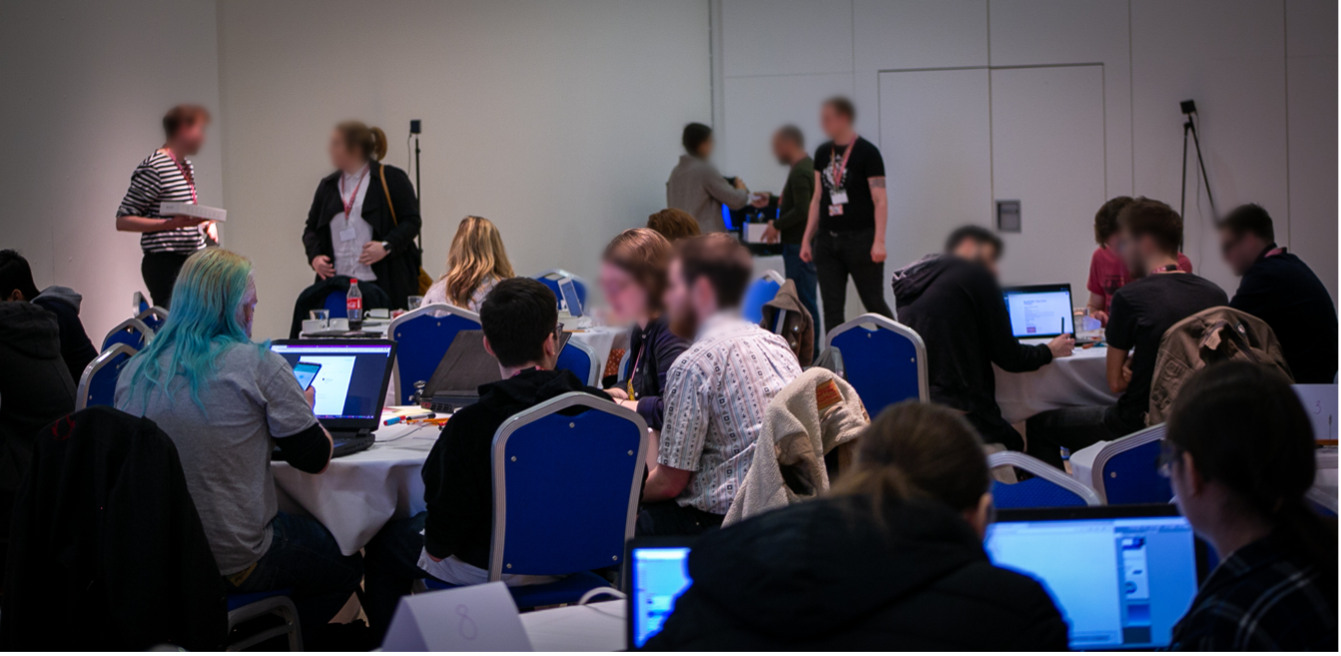
\includegraphics[width=.8\linewidth]{Images/DemVR/Findings/DayOneDemVR.png}
\caption{Day one of DemVR}
\label{fig:DayOne}
\end{figure}

At the end of the event, GardenLife expressed their hopes that \textit{“events such as this and research continuing to deepen our understanding of these issues will help to alleviate the stigma that caused [negative representations] to happen" (W)} presents a series of motivations that participants are keen to learn and educate themselves on sensitive issues. Perhaps unsurprisingly, a sense of competition and prize money were significant motivators for several teams. The first author’s field notes described \textit{“how they [teams] would come up to [first researcher] and say they’re going to win the prize money as their idea is the best” (F)}. While this made for particularly enthusiastic participants, in many ways, it could also be seen to hinder collaboration between teams. Moreover, it was also a potential contributor to why there was little uptake from our participants for using the online platform, which would have made participants’ budding ideas public knowledge.

During our team formation, the first author was getting to know one of the six members who later made-up team Sensory Tide, when they had mentioned how three of the team members had \textit{“got together and had a few meetings, but [their] idea is top secret. [they’re] not gonna share it till we have to” (F)}. Teams’ secrecy in their ideas constrained their willingness to share their ideas publicly before the two-day hackathon in fear others would copy or otherwise be influenced. Similarly, the team that dropped out during team formation had similar concerns of revealing their idea to the extent of questioning \textit{“who owns the intellectual property” (F)} of the idea. 

To provide engagement for people with dementia and care partners, we set up our ‘pre-engagement phase’ that included an online platform, and in-person workshops. As we described in our recruitment, only one of the twelve participants who signed-up to our online platform (Ideaboard) was not a designer/developer. Our one care partner – Denis, was motivated to share his experiences of his father’s dementia hoping outputs of the event would provide \textit{“published prototypes [he] can use [with his father]” (I)}. As Denis continued to comment on the Ideaboard ideas, he would express limitations in people’s ideas saying:\textit{ “my father is too old to use social media” (I)}, or \textit{“my father wouldn’t understand how to navigate in VR” (I)}. In these examples, Denis was advocating on his father’s behalf to make sure his father’s differences may be considered in future VR outputs. Although Denis felt comfortable to share his experiences, several participants without experience of dementia sent emails asking for advice on their ideas before they submitted as they were worried, they would be \textit{“embarrassing [them]self”} from their lack of knowledge around dementia. 

\begin{figure}[htp]
\centering
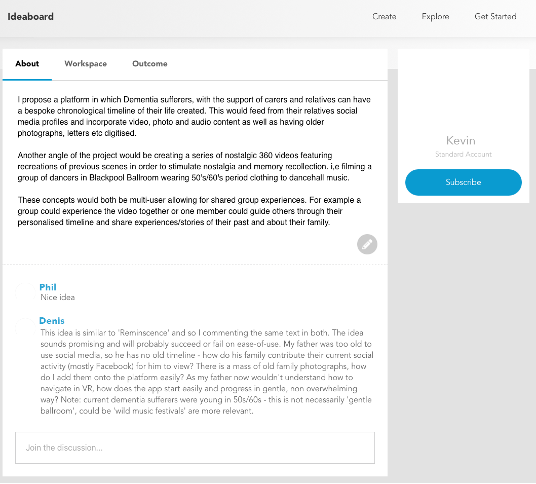
\includegraphics[width=.8\linewidth]{Images/DemVR/Findings/IdeaboardDemVR.png}
\caption{Denis commenting on shared ideas on Ideaboard}
\label{fig:DenisIdeaboard}
\end{figure}

While they expressed, they’d \textit{“really love to be involved and help to make a difference”}, the sensitive nature of the topic at hand made some participants question their ideas and hope that they \textit{“hadn’t got the wrong end of the stick”}. Similarly, the first author’s field notes indicate that “\textit{participants seemed anxious or uncertain if they’d be saying the right thing [online] which might be why they didn’t engage” (F)}. Although several teams felt uncertain to share their ideas or take part in the online platform, participants were still motivated to take the time and conduct research before the event, whether that was GardenLife \textit{“reading VR and dementia papers” (W)}, or how Augmented World had sought guidance from a Dementia Advice Centre about VR as a potential viable technology for people with dementia. Additionally, our planned in-person workshops co-organized with a local dementia café raised concerns for participation when \textit{“no-one signed up to our workshops... CEO of the café just notified me and asked if we should cancel the [the workshops]” (F)}. From the first authors field notes, at the time, they felt \textit{“perhaps members [of the café] are no longer interested in VR work anymore”}. However, even if so, the research team received nine emails after the event from companies/individuals asking if any ideas had gone into \textit{“production”} or any of \textit{“the outputs from the event are in digital form”}. 

Many of these companies specialised in providing \textit{“care across a number of homes”} but reached out looking for cheaper solutions. Participation was scarce in the pre-engagement phase which initially presented that\textit{ “perhaps people are no longer interested in VR?” (F)}, and while this may have been the case for our workshops (that we discuss in our discussion), Denis’ motivation and companies interested in what the event had created suggests maybe the lack of support to learn dementia prior event hindered participants motivation to engage online. This theme describes the motivating factors influencing participants to take part in the hackathon. While there are examples of personal and educational motivations behind taking part, this themes also raises concerns about the type of incentives expected in a typical hackathon event. For example, though prize money motivates taking apart, it hinders the sharing of resources and knowledge between teams as this may affect the competition outcome. However, although our event may not have gained as many participants as it did without prize money, there are some instances of teams’ going out of their way to initiate conversations with care partners or sharing their personal experiences in the hope to have a say on the hackathon’s VR outputs, indicating that at least some of our participants’ motivations were pro-social in nature.

\subsubsection{Participant implementation of these new understandings}
\label{ThemeOne:subthemeTwo}
In our pre-hackathon stage, the submitted ideas formed an initial picture of how prospective participants viewed dementia – for instance, through their idea helping to \textit{"making them [people with dementia] feel more independent"}, or to \textit{"help calm the mind[s]"} of people with dementia \textit{(I)}. Although multiple participants used terminology no longer accepted in best practice in dementia, such as \textit{"sufferers"}, and\textit{ "patients" (I)}, the design ideas uploaded suggest these terms are not intended to stigmatize. For example, a participant from team World Share suggested ways for VR to \textit{"guide sufferers through daily basics" (I)} in order to reduce the effects of memory loss by having VR technology allow them to repeat tasks such as \textit{"basic cooking, making a cup of tea" (I)}. Although these terms were being used early in the two-day hackathon as well, through engaging in conversations with facilitators, and through introducing resources such as the DEEP Guide \citep{diaries_deep_2020},  participants changed their language and used more respectful, person-centered terms. In the same vein, many early iterations of participants’ ideas promoted 'treatment', 'fixing the disease' and ways for technology to improve a person's memory or other deficits \citep{hendriks_valuing_2018}. Throughout the event, several teams, particularly those made up of undergraduates, expressed their interest in learning from academic papers. For example, Mindful Forest described \textit{“a research paper about this care home in Sweden, that took outpatients in the forest and found patients communicated more and remembered more about it” (P)}. This paper inspired them to create a forest environment for their final design.

\begin{figure}[htp]
\centering

\includegraphics[width=.8\linewidth]{Images/DemVR/Findings/MindfulForest.png}
\caption{MindfulForest influences from Sweden dementia forest research}
\label{fig:MindFulForestResearch}
\end{figure}

While facilitators assisted in suggesting particular papers or articles, it led to GardenLife initially designing for ways to link memories to locations, to develop and ideate on social complexities of feeling \textit{“silly” or “scared” of using VR – and to find a solution of “easing [the user] into the experience” (P)}. Through initial facilitation, conversations, presentations and inspiration packs, World Share described their interest in understanding the\textit{ “the challenges, accessibility, interactivity, and limitations around dementia care the people around people with dementia” (W)}.

Additionally, teams’ design decisions were influenced by conversations with stakeholders before and during our hackathon, such as Howard’s Q\&A, discussions on Ideaboard, or reaching out to caregivers outside the event’s network of people. For example, Augmented World designed for AR rather than VR based on advice from a Dementia Advice Centre, which suggested: \textit{“VR might be quite frightening…and with it being a bigger adjustment mentally with them living in a reality they don’t know what is real or not” (P)}. Similarly, Michael – a team member from Sensory Tide - engaged with Denis via Ideaboard to gain a richer understanding of dementia from a care partner’s perspective. Denis highlighted ethical and financial concerns for Michael’s proposed idea on Ideaboard: this was to create\textit{ “full-dome projections” (I)} as an alternative to \textit{“wear[ing] VR headsets” (I)}. The care partner and the designer engaged in conversation on the platform and raised concerns about projection domes’ practicality for care homes. The care partner pointed they are \textit{“\$13,000 as base price” (I)}. The team shifted their course from here, and their final idea was by developing light-weight DIY solutions through the use of Google Cardboard. During Howard’s Q\&A, VRHallucinate started to link prior knowledge of hallucination research and aligned it with Howard’s shared experience of hallucinations he has been having recently. While the team initially identified similarities between their understanding and Howard’s stories, when he opened up about how his friends\textit{ “disappeared, and only three people still keep in touch” (P)}, the team altered their idea, shaping it instead about being how VR could \textit{“teach [people with dementia and their care partners] to experience these visual uncertainties and inconsistencies, by playing a problem-solving game that will manipulate and change as you play to signify a change in hallucinations” (W)}. 

\begin{figure}
\centering
\begin{subfigure}{.5\textwidth}
  \centering
  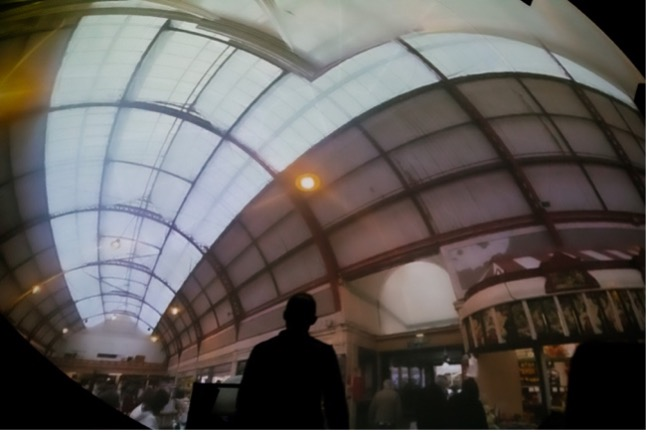
\includegraphics[width=.8\linewidth]{Images/DemVR/Findings/DomeProjection.jpg}
  \label{fig:Dome}
\end{subfigure}%
\begin{subfigure}{.5\textwidth}
  \centering
  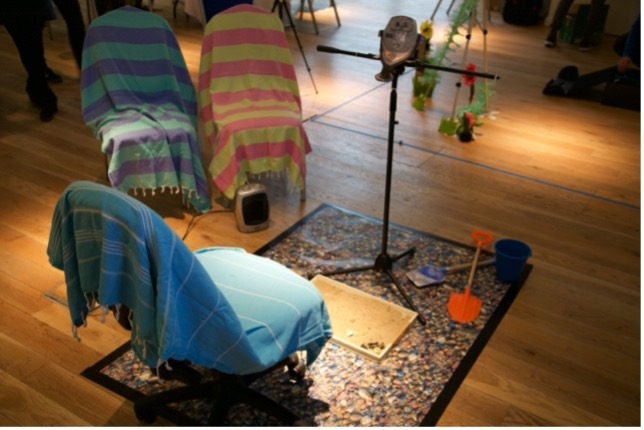
\includegraphics[width=.8\linewidth]{Images/DemVR/Findings/SensoryTideDIY.jpg}
  \label{fig:senosryTideDIY}
\end{subfigure}
\caption{Change in Sensory Tide's VR technology}
\label{fig:SensoryTideDesignProcess}
\end{figure}

While participants demonstrated new understandings of dementia and how they may design for this care context, adopting this critical approach in their design proved challenging for the teams. In fact, the only teams who demonstrated this critical sensibility are the ones populated by experienced dementia researchers. The two winners of the hackathon - ChatterBench, Sensory Tides and team VRmotion could pull from their successes and failures in the area and critique their ongoing design decisions. For example, Sensory Tides took inspiration from the many language guides around dementia and considered what that would mean for the term ‘Virtual Reality” (see table 3 for final idea). Aware of the social complexities that people with dementia may face with defining their reality and the concerns that earlier academic work had with the terminology surrounding Virtual Reality, the team designed for continued reassurance through the technology instead. Instead of the term VR, they describe their experience as a “magical viewfinder” (P) along with giving calm and helpful suggestions of how users may use it: either by leading the experience through the viewfinder or “lean[ing] back away from the headset and join everyone else relaxing on the [virtual] beach” (P). 

Similarly, Chatter Bench and VRmotion began to question some of the more ethical and social challenges of designing within this space. The teams questioned, “How are you going to fit [the experience] into the [care home’s] schedule?” (P), or VRmotion considering “who controls [the experience], why would the person with dementia control it?...How would a facilitator involve themselves into the experience?” (P). In the teams’ final presentations, Chatter Bench raised concerns that their idea may add “strain on the family and resources” (P) in order to create the 360-degree worlds that people with dementia and care partners may want to share together – to the point that Chatter Bench presented future ideas of more social and community-led curation methods to generate a variety of environments in the “hope it will scale” (P). Although the event provided participants with curated research papers, ‘snippets’ of the lived experiences of people with dementia, and resources such as the DEEP Guide, these reflections can only offer examples of best practice rather than develop genuine understanding and relationships that may mirror the type of experiences the researchers suggested they had.  The extent to which we can support participants to both learn about a complex issue and apply this new knowledge to design within the traditional hackathon structure warrants further consideration. We return to this reflection in the discussion. 

\subsection{Reworking participants' conceptualisations for design}
\label{LearningEvent:ThemeTwo}
Through the event, I had hoped to engage with people with dementia and care partners in order for developers/designers to have the opportunity to gain insight into what priorities or interests they should keep in mind when designing their shared VR experiences. However, as I have described in the chapter, I did not manage to involve care partners and people with dementia in the ways that I had hoped. As a response, the following subthemes describe the subsequent consequences of a lack of engagement with lived experience, where teams had to adopt different approaches to design for an absent user. Furthermore, I discuss the outcomes of designing for users who are not present, highlighting how designers returned to established ideas of deficit models of dementia. 

\subsubsection{Constructing the absent user}
\label{ThemeTwo:subthemeOne}
Teams’ ideas shifted over the course of the event as their interactions with facilitators, inspiration packs, and Howard unfolded; we noted that participants often focused on particular comments made by speakers who discussed their experiences with people with dementia. The interplay between the stories, resources and conversations scaffolding the event helped to create an initial understanding of what it might be like to live with, and design for, dementia. However, by having a lack of people with dementia and care partners at the event or through engagement on the online platform, a number of teams pictured the person they are designing for on Howard’s experiences of dementia that he shared in his 15-minute Q\&A. For those teams, Howard became a pivotal resource, and a somewhat static personality they were designing ‘for’. The ways in which teams reacted to Howard’s experiences varied. Team Garden Life changed their design approach in response to Howard's hobbies and interests: their initial idea centered around "a journey through the story of your life using different media that links memories with locations'.” They stated that “The experience can be customized by family, so that the focus is on either neurological rehabilitation or reminiscence" (I). 

\begin{figure}[htp]
\centering
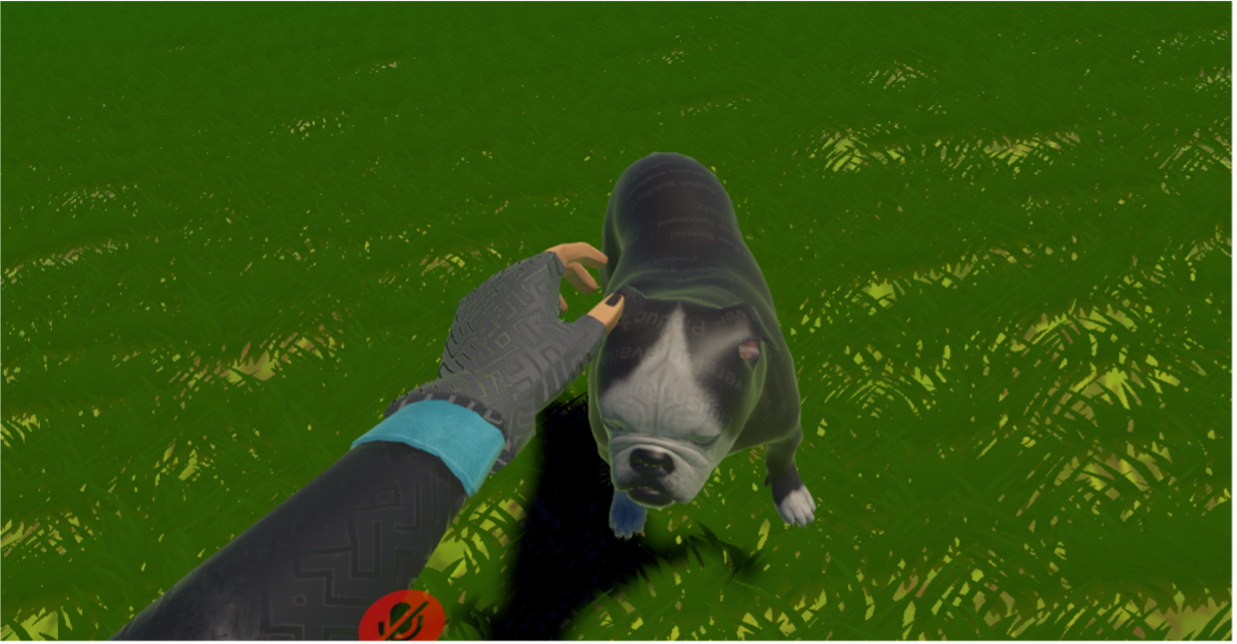
\includegraphics[width=.8\linewidth]{Images/DemVR/Findings/GadenLifeVR.png}
\caption{Garden Life VR dog companion}
\label{fig:GardenLifeDog}
\end{figure}

In response to Howard’s Q\&A, the team developed a virtual reality ‘garden’, with a feature that allowed the user to interact with a virtual dog. In the WhatsApp group chat, the team state that they "found it interesting [Howard] has a pet dog" (W). This led to the team reflecting on how people living in a care home may not get that opportunity, but that "having an animal to care for seems to help people in a lot of ways' (W)'; and the team felt a virtual dog could help with loneliness. As the team developed the garden environment further, they built customisability options: “you can change its breed, colour and name of the animal" (W). Similarly, while Mindful Forest didn’t focus entirely on Howard’s experience, Howard’s experiences provided an opportunity to expand their current understandings of dementia as they “realized [they] actually don’t know as much [about dementia]” (W). In response, the team’s final idea featured “family members adding various pictures from holidays when they were young, so it would help in remembering if they forgot about their grandson or grand-daughter” (P). While the team prioritized their experiences of dementia where “I still remember the day when my Grandma no longer recognized me” (P),  the team were inspired to enhance their social features after being “surprised that all of Howard’s friends left”.  While basing design decisions on personal stories, or on Howard’s is not necessarily harmful, the lack of interaction with a variety of people with dementia limited the space for creativity and exploration, and instead presented Howard’s or participants personal experiences as a ‘one size fits all’ persona for dementia. Further, our event overlooked involvement of care partners, health care providers and friends who may be involved in the ecology of care which limited teams such as Chatter Bench describing they ‘have no understanding of how a nursing home really works”. 

\begin{figure}[htp]
\centering
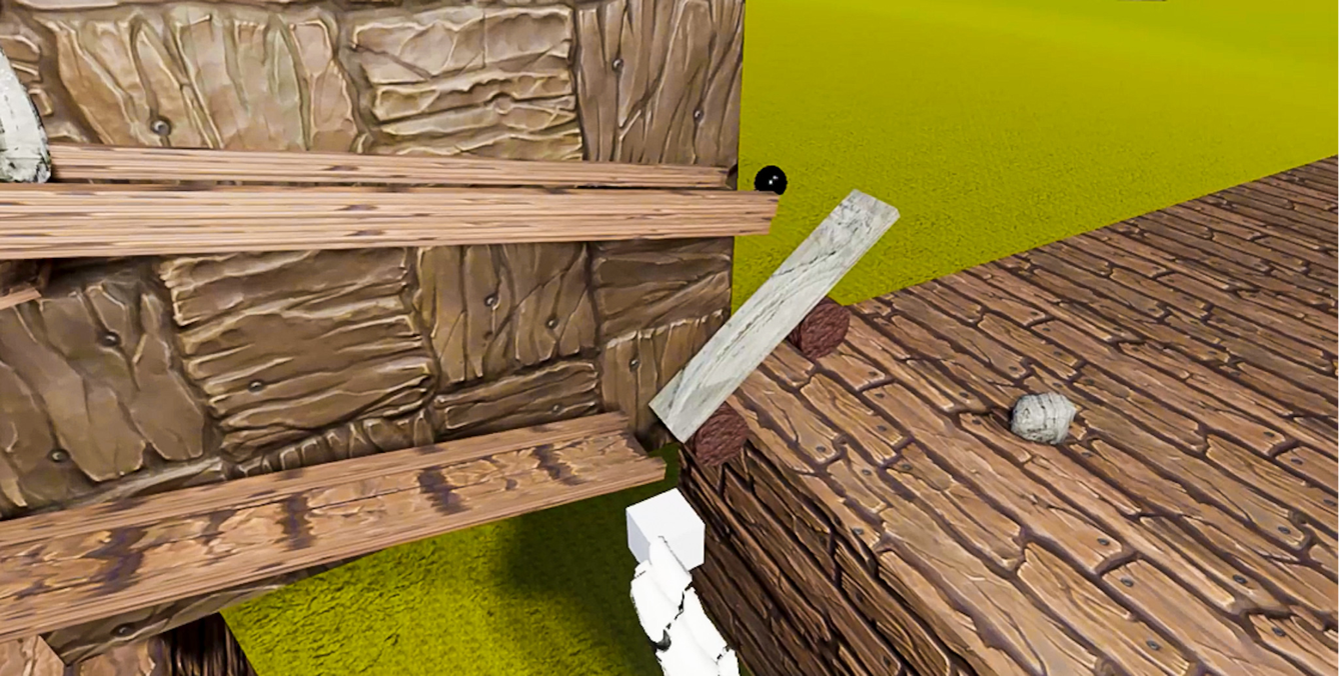
\includegraphics[width=.8\linewidth]{Images/DemVR/Findings/VRHallucinate.png}
\caption{VRHallucinate educational game on hallucinations}
\label{fig:VRHallucinateDemo}
\end{figure}

For the most part, teams' initial ideas as outlined in the methodology are centered around cognitive training and reminiscence, except for three teams – VRMotion, Sensory Tide and Chatter Bench. Perhaps coincidentally, these three teams had at least one researcher with a background in working with people with dementia who could not only draw on their prior experiences, but also had extra insight into current research in HCI and dementia care. The three team’s shared design focus of \textit{"being in the moment"}, or \textit{"celebrating what abilities are left"} are not particularly novel contributions to dementia research, but they speak to the participant’s knowledge of the best practice in care. With that said, even though Sensory Tide and Chatter Bench won the final prizes, they still struggled to construct an understanding of who the user might be. During their final presentation, Sensory Tide presented a set of personas that often abstracted the user and were prone to stereotypes such as: \textit{“Mary: can often get confused or lost if left alone” (P)} and \textit{“Ben: has anxiety and depression as a result of his diagnosis (P)}. 

Although personas can be useful for designers to connect with the people they are designing for, it shows that even the winning teams were limited to representing the person with dementia as a set of stereotypes based on their diagnosis. Although Sensory Tide used the personas to \textit{“help us decide who we are actually designing for”}, for reasons similar to Chatter Bench, they found it \textit{“hard to figure out what to design because [they] can’t ask the user” (W)}. This observation goes a way towards highlighting the value teams placed on engaging with end-users in the research, and highlights what is at the centre of this finding: the perceived importance of engagement between designers and stakeholders. In our final sub-theme, we describe the continued effect that the lack of stakeholder involvement had to designer’s creativity as they prioritized risk aversion as opposed to exploring a range of possibilities that people with dementia may want to experience. 
\subsubsection{The trade-off between autonomy and safety}
\label{ThemeTwo:subthemeTwo}
Some teams raised concerns regarding how best to represent an appropriate environment virtually for users with dementia. This often resulted in taking an inherently ‘safe’ design approach in order to reduce any 'negative' or 'confusing' experiences, thereby ensuring neutral or positive emotions. For example, team Chatter Bench were conflicted in \textit{"how [to] represent the person living with dementia [in VR]" (W)}. The team's idea is a ‘VR skype call' where both participants would be present in a 360-degree video on a bench in a park. Members of this team were attuned to the technical aspects of design, having worked in VR over the past five years, where the concern of the illusion of embodiment and the representation of the user's body has been regularly discussed \citep{nakamura_virtual_2019}. For example, when discussing the possibilities of designing avatars for the VR environment, they worried that, \textit{"the other [avatars in the environment] will look like a scary apparition or, you know some floating smiley head" (W)}. To tackle this concern, the team removed the virtual avatars and transmitted only the online voices between the two users. The team suggests their decision was to some extent a trade-off: when you are already \textit{"placing a headset on somebody with dementia”} (and therefore causing some discomfort in all likelihood), \textit{“you don't want to take it to a further extreme when you're showing, magic hands popping around or magic heads" (W)}. 

\begin{figure}[htp]
\centering
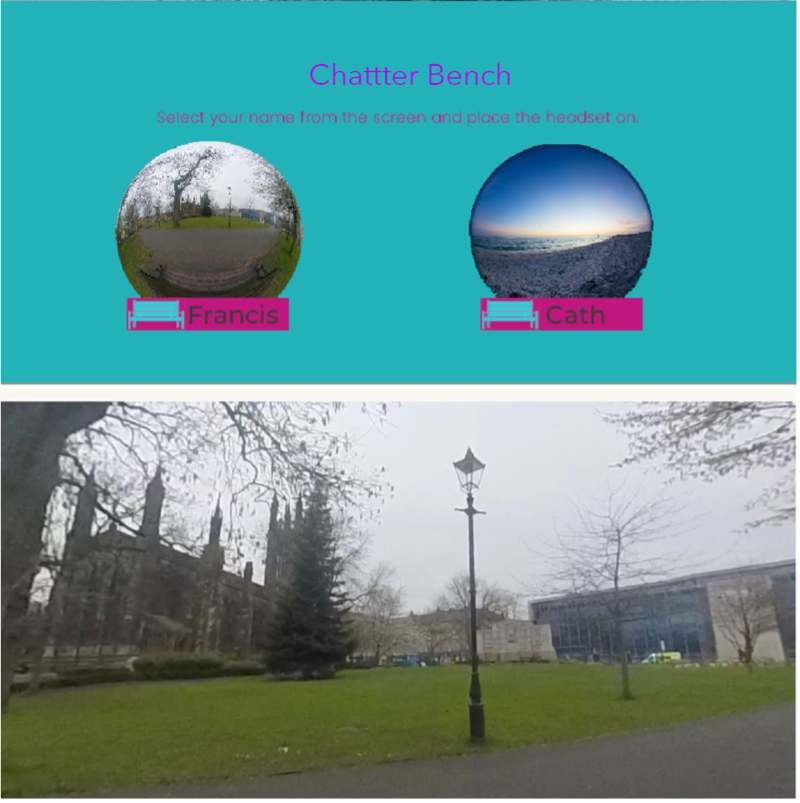
\includegraphics[width=.8\linewidth]{Images/DemVR/Findings/ChatterBench.png}
\caption{Chatter Bench shared VR locations}
\label{fig:ChatterBenchDemo}
\end{figure}

Despite ‘magic hands’ and ‘floating heads’ being common way to represent the user in VR, the team remained skeptical of this approach due to the common conception of people with dementia as unable to decipher what is ‘real’, and what is not, in both real life and in VR. Similarly, team Mindful Forest, state that they originally \textit{"planned to add fantasy elements to our idea. But due to learning about other symptoms like hallucinations, we, therefore, had to change it to be more realistic, because we don't want to cause any problems for people with dementia" (W).} Both teams were focused on the person’s safety, deciding that this was more important than designing for autonomy or ideas of abstract aesthetic engagement. In both instances, designers took the decision-making process out of the user’s hands by removing fantasy elements or bodily representation in VR to prevent harm. While user’s safety is a priority in any form of design process, removing the option of switching features off or on can be argued to restrict the expression of individual differences and limits the potential autonomy a person with dementia may have over the experience.

Many teams whose ideas sought to involve care partners, families or friends would often make design decisions that shifted the responsibilities of setting up the technology to the caring role. Again, while this may be useful or even preferential for some, it may also result in a loss of agency for the person with dementia. For instance, team Chatter Bench stated that if their VR experience was implemented into a care home, then scheduling of the VR 'Skype calls' need to consider \textit{"fitting into the schedule of the care partner as well" (W)}. The team realized that a diagnosis of dementia often brings along with it a shifting of responsibilities, with these being placed instead upon others such as their care partner, potentially further eroding the autonomy of the person with dementia and contributing to caregiver burden. 

\begin{figure}[htp]
\centering
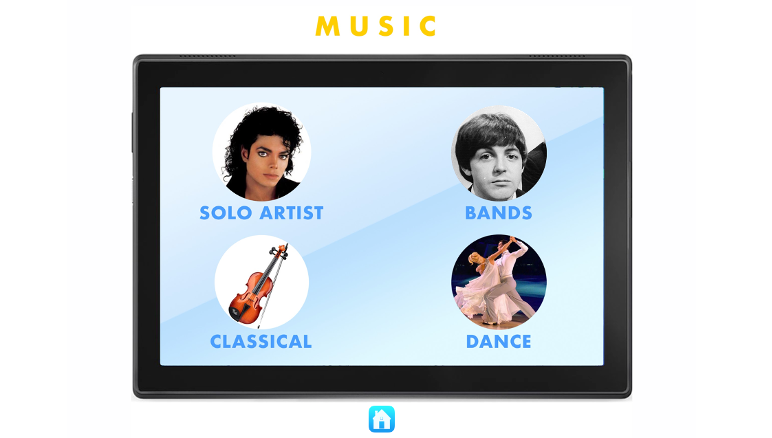
\includegraphics[width=.8\linewidth]{Images/DemVR/Findings/WorldShareUI.png}
\caption{World Share's UI interactions}
\label{fig:WorldShareUI}
\end{figure}

Alternatively, team World Share focused on their interactive app consisting of events, family and friends’ recordings to be as customisable as possible to \textit{"approach the widest possible audience" (P)}. World Share's approach wanted the user to have as much ownership and agency when using their VR system as they argued \textit{"just because you have dementia, does not mean you don't want to learn. You want to be able to explore these things" (P)}. Although this idea encourages customisability to tailor the system to the user, it could also be argued that placing all the decision-making processes on the individual may also hinder or overwhelm the user through exploring the system. In sum, the majority of teams found it challenging to design VR as a shared experience particularly when trying to place responsibility on who drives the experience – the person with dementia, or the care partner. However, while they still found it challenging to navigate the space of shared VR experiences, Sensory Tide designed their VR experience with reference to experiences both of families living with, and those with dementia. In this instance, as the person with dementia controls the movement of the VR headset, this drives the experience for not only themselves, but projects what they are seeing into the outside space of the room for the family to see.  

Similarly, VRMotion designed a series of VR activities such as “songs to sing along to, guess the place, solve the riddle or even share jokes”, and considered the collaborative decision-making needed to ensure continued participation within the care home. This is done through giving the staff member the responsibility as a facilitator to “pull a lever on a [VR] slot machine, which will show a random task. [Then] people with dementia and the facilitator will work together to complete the task”. These examples highlight difficulties that may occur when designing for decision-making, where the two extremes are to either place all the responsibility onto the care partner through risk-averse approaches or giving full responsibility to the person with dementia to aid their autonomy. However, in some cases, such as VRMotion, they considered ways to maintain reciprocal interdependent relationships where the person with dementia is part of the decision-making process resulting in a more collaborative experience through not only the experience, but the set-up and responsibility of actions. 

\section{Discussion}
\label{sec:Discussion}
The analysis presents the nature of participation from team members, and the impact of structural factors of the event on design outcomes. I explore the different reasons participants were motivated to participate in the hackathon. Motivation for involvement ranged from personal experiences to learning, albeit collaboration between teams being hindered by competition. I also compare participants’ ways of incorporating their new understanding of dementia into their design ideas to highlight critical differences between those with and without extensive experiences of dementia. Finally, as an outcome of the lack of engagement of people with dementia and care partners in the event, the second theme describes how teams attempted to design for the absent user through different means, showing that teams often prioritised safety over autonomy when uncertain if VR features may cause psychosocial risks. Overall, these findings raise some important considerations for design events such as best understanding participant involvement, designing for the ‘absent user’, and redefining what collaboration may be between different communities, which I further discuss in the next section. Considering the analytic findings and existing literature on reification in design, collaborative design events, community building, and meeting participants where they are, I provide a series of considerations that suggest researchers and designers to consider ways to mitigate stereotypes, improve recruitment processes, and future approaches to re-design hackathons. 

\subsection{reification, experience \& designing with and for stereotypes}
The transformation of complex individuals, groups, communities, processes, and systems into manageable constructs to inform design has long been noted in HCI. Such conceptualizations are often referred to as creating or using boundary objects – that are \textit{“entities that enhance the capacity of an idea, theory or practice to translate across culturally defined boundaries” (pg. 71)}\citep{fox2011boundary}, which are adaptable across application areas, but which are also solid enough to represent one ‘thing’ or meaning across these areas too. The participants, working with an idea of their own end users as ‘sufferers’, or as those dealing with instrumental cognitive problems wholly aside from the felt experience of their own dementia, were working with a boundary object – the \textit{“Person With Dementia”} - which was manageable for a weekend’s design work, but may have shut down possibilities for greater creativity and wider representation. While I suggest people with dementia should always be involved in conversations in design settings, given the challenges encountered by participants when reliant on a set of resources to construct their person with dementia, I suggest three considerations to \textbf{mitigate stereotypes} for researchers and designers:

\subsubsection{1. Not everything needs to be a solution}
\label{sterotype:One}
Living with dementia can lead to varying cognitive abilities which can make daily tasks challenging and potentially further heightened by design choices within the environment or by the way people act towards someone with dementia. Engineering and design disciplines are often focused towards problem-solving methodologies. This may account for why our hackathon resulted in a high number of solution approaches to tackle challenges that people with dementia may face. For instance, Garden Life \textit{‘found it interesting that [Howard] has a pet dog’}, and so go about inscribing this already existing reality into a technological solution – they create a VR dog interaction where the user \textit{‘can change its breed, colour and name’}. This is an almost exact translation of a reality offered to the participants as an example, but while the team acknowledge that ‘having an animal to care for seems to help people in a lot of ways’, they are unable to delve further due to the absence of other people with dementia present, a lack of personal experience, and overall, a lack of time. 

This virtual representation of an enriching human-animal relationship is in stark contrast to existing research on technological approaches to designing animal companionship for older people by \cite{lazar_rethinking_2016}. In this study, older people express a need for comfort and companionship through \textit{‘cuddling and petting live pets’} and wanting a pet that was \textit{‘warm, soft’}; which promotes social opportunities for getting out and about; and a reciprocal relationship. This isn’t to say that Garden Life’s idea was unsuitable, or that VR experiences cannot at all provide these sorts of qualities; but that our participants were disadvantaged by time and by lack of engagement with ‘real’ participants – and as such, were able to provide only a shallow exemplar which might have been much richer. It is also worth considering general depictions and understandings of ageing and dementia as a ‘problem’ facing society, which can also influence design. 

Pullin argues that not all design challenges in disability are \textit{“best described as problems to be solved”} (pg. 41) \citep{pullin2009design}. Further, for issues that are not easily defined as problems, we risk under examining issues that could provide important changes for the people we are design with and for. Although our conventionally-structured hackathon can be seen partially responsible for influencing a problem-to-solution approach \citep{hope_hackathons_2019}, design approaches such as personas and scenarios are rather static and often designed to elucidate problems that designers and developers may want to tackle \citep{cutting_can_2019}. One alternative designer’s may consider is expanding persona-like approaches to be more reflexive and experimental through their design workflows. For example, \citep{leong2021experiential} describes open-ended personas that were designed with the intention to have more interactive and embodied purposes. In this way, a 2D written persona is developed to have material imagination through tangible belongings such as desks, calendars, books, and photos of the persona. In this way, the designer is introduced to new interpretations and define their own unique meanings towards the experiential persona. Therefore, while traditional methods that were implemented in our event limited designer’s experimental and openness, we encourage designers to take these traditional design approaches to understand our participants and reimagine ways to support a full range of embodied experiences. 

\subsubsection{2. Looking beyond one's abilities}
\label{sterotype:Two}
When we design for people with dementia and others in marginalised populations, we often place emphasis on abilities and the ways technology may provide improvement in abilities. For instance, reminiscence therapy for memory problems \citep{astell_stimulating_2010}, exergames for motor deficits \citep{unbehaun_exploring_2018}, and tracking products for ‘wandering’ \citep{kearns_attitudes_2007}. While this work is beneficial, focusing on people’s ability runs risk of overlooking diversity among people who share the same deficits. Within our hackathon, focusing on the cognitive deficits that come with a diagnosis of dementia, led to some participants’ solutions being risk averse. This is described in the final sub-theme, where the autonomy of the user was pitched against the potential risk of infringing upon their safety or their comfort: Chatter Bench were worried about the ‘strangeness’ of bodily representation in VR; while Mindful Forest decided against the addition of any fantasy elements to their design response for fear of triggering hallucinations. While the safety and comfort of our participants should be paramount in our minds as we design new technological responses, a heightened focus on risk might quash creativity, remove any room for individual differences in user experience, and further limit the expressive and aesthetic potential of the technology itself. 

It has been noted in applied psychological research that the presence of risk limits participants’ creativity when critiquing, problem finding, and see new patterns \citep{amabile_social_1990}; but in design, following these risk-averse approaches may lead to the cyclical perpetuation of stereotypes in design features and interactions. By presuming that people with dementia are unable to handle features such as ‘floating smiley heads’, or ‘fantasy elements’, we run the risk of restricting the range of possibilities for users who don’t feel represented by this range of interaction; further to this, we may influence future designers to work solely within the range we’ve defined. While features such as fantasy elements, or floating heads may increase anxiety, or heightening confusion within the VR experience, restricting design based on potential shared deficits has numerous knock-on effects – for one thing, the same practice often leads to excess disability in residential dementia care \citep{keady_involving_2007}. 

It is of course true that many people with dementia will find their abilities deteriorate to a point at which they are unable to make decisions for themselves, where they may engage in dangerous, aggressive or self-destructive behaviour, or where they may cease to communicate entirely \citep{baumgart_summary_2015}. It’s also true that many people with dementia deal with problems with cognition and perception which may make new experiences stressful or otherwise challenging \citep{west_operationalising_2017}. However, many people with dementia are also able to sing, dance, act, clown, play games, write, engage in their own families and communities, and even continue meaningful work; they may engage in such activities on a continual basis, but perhaps also on a fragmented basis \citep{landmark_couples_2021}. 

\subsubsection{3. Disseminating research outputs}
\label{sterotype:Three}
Disseminating our research in less ‘static’ ways to offer participants new explorations into ethical and embodied topics of dementia is an opportunity to further mitigate designing for stereotypes. In the last several years, we have seen a gradual shift in disseminating dementia work, such as the theatre play Cracked that responds to promoting inclusivity and engagement to tackle stigma \citep{kontos_raising_2018}. This recent work resonates with the ongoing drive towards using film for public health and cultural awareness in educational programmes to elucidate in-class discussions \citep{botchway2017films}. To have improved the dissemination of our event, I could have done this in several ways. The first would have been to provide each team with workbooks \citep{mucha2020co} to fill in over the event. While I documented the design processes through WhatsApp group chats, audio recordings, and field notes, they are challenging to disseminate. 

They require significant context to understand the individual pieces of data. Instead, providing workbooks that structured documentation could have provided the opportunity to publish design processes (if teams chose to) online to disseminate the team’s shifting representations of dementia. Second, hiring designers, filmmakers to develop a set of resources inspired by the team’s final ideas that could have been shared online, particularly with the organisations and individuals who reached out post-hackathon. Therefore, to get the public to engage with the more sensitive and complex topics, taking an alternate approach to presenting our work such as through theatre, zines, and other creative arts methods may result in a set of work that provokes similar understandings that researchers aim to gain from working alongside people with dementia.

\subsection{Facing actual reality: Unplatforming and participant disinterest}
\label{Unplatforming}
Previously, I focused on how participants’ conceptualisations of people with dementia led them to make assumptions about the population, which may have restricted their creativity and perpetuated stereotypes. However, what’s also clear about this project is that our configuration of the hackathon gave rise to certain challenges. Prime among these was the extent to which people with dementia were meaningfully engaged in the event itself. As noted above, I tried to involve people with dementia (and their care partners) in three ways: 1) through planning workshops through a community partner with whom we’ve worked several times, 2) as full participants during the day itself, and 3) as participants on our online platform, Ideaboard. 

The former two routes failed, as no person signed up through our community partner; the latter route saw some engagement, but ultimately much less than we had hoped. Late in the planning process, we invited Howard to share his experiences and engage in a Q\&A with our participants, in order to ensure that our attendees had an opportunity to engage with at least one person living with the condition around which the event was centred. We also ensured that participants were provided with information materials drawn from best practice guidelines on working and designing for people with dementia. 

Despite growing research has indicated, that older adults capably make rich use of technologies such as e-mail and Youtube \citep{sayago_telling_2010,sayago_everyday_2011}, \cite{hwang2020exploring} work with people with dementia and care partners found “that technological support needs may vary over the appropriation process” and will often require the support from care partners who are also aware of the changing cognitive perceptions of the person with dementia overtime. 

Although Ideaboard was not created solely for older users (whom we envisaged as the people living with or caring for dementia who might be interested in our hackathon), it was configured with them in mind, and it is true that more familiar technologies might have been used in soliciting the views and opinions of participants with experiences of dementia.  Aware of the ramifications of an online only interaction through Ideaboard, we did seek to carry out a series of workshops in our pre-hackathon engagement stage with a local partner. However, during the recruitment stage, no members signed up to any of the workshops. In the following sub-sections, we provide a set of future considerations for \textbf{recruiting} and involving marginalised populations in future work:


% \subsubsection{1. Meeting your participants where they are}
% \label{participantsWhereTheyAre}
% Instead of designing additional online platforms, we suggest asking participants what platforms they would like to use for engagement. Not only does this reduce development costs, but this also provides the opportunity to understand the communication processes your participants are familiar with. One approach we might have adopted would be an ‘Unplatformed’ approach to the design of the pre-hackathon experience and recruitment stage. Unplatformed design is a model for the appropriation of social media technologies, that pays particular attention to the implications of the individual features of social media in respect to coordinating participation in specific contexts \citep{lambton-howard_unplatformed_2020}. We might have reduced barriers to engagement and ensured better representation of the views of our participants by coordinating participation on the technologies that they were already comfortable with (e.g., Twitter, Facebook, and other media platforms). Although we knew that some members of the community whom we would have liked to have reached used these platforms, we were seeking an additional ‘string to our bow’ by piloting the use of the Ideaboard platform. Nevertheless, in this case, it hindered rather than increased participation. 

% However, it should also be noted that utilizing solely digital methods to facilitate recruitment and engagement could be limiting for some participants facing significant marginalization. For instance, \citep{lazar_safe_2019} describe how even inclusive initiatives centred around the involvement of people with dementia may silence voices that offer less "polished stories" or those who are nonverbal. \cite{dai2020making} describe that while online interactions provide an enjoyable and beneficial interaction for the person with dementia, it contributes to a burden and the need for the car partner to provide \textit{“responsive, continuous, and knowledgeable support|” (pg. 46:24)\citep{hwang2020exploring}}. 

% Moreover, we should consider ways to invite and involve participants in the research processes and recruitment stages to help ensure agendas and processes to engagement are more closely aligned with the participants. To this extent, participant-led research may offer understandings into new, more impactful ways our research be of benefit to communities beyond academic publications. Alongside, researchers should continue to provide additional context for their recruitment methods when working in sensitive settings to generate a set of knowledge on the challenges and possibilities of participant engagement in this area of work


\subsubsection{2. Fostering participation through relationships and topic training}
\label{TopicTraining}
During the recruitment stage for inviting people with dementia, I leaned on the expectation that the CEO would describe hackathon and VR topic to members of the dementia café that I had already worked with in the past. However, in this way, without building training and learning, the lack of investment by people with dementia may echo \cite{hwang2020exploring} reflections of if technology \textit{“evokes frustration, anxiety, or sense of vulnerability” (pg. 46:26)}, then resistance to the new technology and idea may increase. In this way, we are guilty of many of the shortcomings levied against researchers who claim participatory work yet don’t involve their participants from the ground up, and don’t schedule in regular check-ins to ensure interests and priorities haven’t shifted. Recent work in public engagement has indicated that, for health research to be truly collaborative, participants must be engaged from the ground-up in setting agendas and priorities. Although I had a long-standing engagement with our charity partner, I overlooked that their priorities might have changed.

Although VR enticed developers and designers to take part in designing for a new and upcoming piece of technology, supporting communication and training before the pre-hackathon stage for people with dementia, developers and designers may have provided confidence and interest for the differing communities. For instance, while the findings describe Augmented World reaching out to care partners through a Dementia Advice Centre, other teams expressed an uncertainty in their knowledge on the topic. While we provided guides and resources to support their understanding of dementia, facilitating early engagement between designers, developers and people with dementia in dementia cafés and alternative locations may have provided more meaningful interactions and relationships to form over the period of creating the VR experiences that echoes \cite{hendriks_valuing_2018} argument of the importance of relational approaches to inform design decisions. While future work should consider how to educate and support training for the public to reach out to other communities, and to up-skill participants towards understanding the research topic, this may come with additional challenges surrounding motivation and value of participants’ time. While I describe motivation in more detail below, spending vast amounts of time in support and training without clear indication of community outcomes may hinder interest from communities that are already heavily exploited for their free-labour and insights \cite{medina_angarita_what_2020}.


\subsubsection{3. Supporting the ecology of care within the research topic}
\label{ecologyOfCare}
As previously mentioned, although the hackathon was centred on shared experiences for people with dementia, the topic lacked any primary focus on care partners, families, and friends – those who make up the ecology of care for the person with dementia. In hindsight, undermining care partners desires and interests may have contributed to the struggle in recruitment.  \cite{piper2016technological} describes four forms of work that care partners may perform in an online activity such as: social media apps, responding to emails and online browsing. From the four forms, they are processes to assist in the use of technology that provides continuous adaption based on the needs of the person with dementia. The four forms of work are the following: 1) guiding: providing teaching, assistance in online activities; 2) stimulating: through informational, social, and emotional means such as encouragement of exergames; 3) connecting: setting up video, assisting in replying to forum messages, emails; and 4) protecting: to ensure people with dementia avoid phishing attempts, scams, and fake friend requests. Given all the support care partners provide for the person with dementia to stay connected and educated regarding technology, it is no surprise that several studies describe care partners want to promote their agendas and perspectives in the domain of technology and dementia. 

Furthermore, apart from the winning team, Sensory Tides – who designed an experience that could be shared with care partners and provided the space for necessary support for the person with dementia, little attention was given to the values, expectations and needs of care partners. While this was the fault of ours of only prioritising people with dementia within the topic, future work of technologies should continue to consider ways to prioritise both the desires and interests of the person with dementia and their ecology of care. Progressing in this area will mean careful co-design consideration that pays attention to the eclipsing desires and interests of those with dementia and their care partners.

\subsection{Towards a new economy of collaboration for design events}
\label{newEconomy}
\cite{falk_olesen_10_2020} write, in a review of 381 publications referring to hackathons held during this time, that three main motivations for such events are 1) structuring learning, 2) structuring processes, and 3) enabling participation. The authors also differentiate between research with, and research on hackathons, and outline a series of benefits and challenges for both: some of which have already been discussed in our account of our hackathon. One which deserves some consideration due to its frequency in other papers \citep{birbeck_self_2017,johnson_civic_2014} is that hackathons have\textit{ ‘limited sustainability and implementation of hackathon outcomes’}. This paucity of workable outcomes is in stark contrast to the resources that are often ploughed into hackathons – for example, our hackathon, which drew on public funds and involved the labour of several highly skilled individuals over several months, cost £5,000 to hold. While \cite{falk_olesen_10_2020} note that such events target \textit{‘real-world’ problems, ‘facilitate new research projects and publications’, and help to ‘[imagine] citizenship in new ways’}, they also note that ‘\textit{it can be difficult for peer researchers to evaluate and build upon hackathon outcomes if the circumstances in which the outcomes were created are not well-documented.’}

When such events are predicated on ‘making things better’ for marginalized communities with no clear pathway to actually do this; with limited participation and high barriers of engagement for these communities; with budget and university pathways to compensate the designers and developers but not the population themselves; when these events overwhelmingly focus on the problems, discrimination and indignities faced by people undergoing significant challenges: then marginalised people become the currency with which we trade. Before we describe our vision beyond hackathons where we describe companion communities, within this section, we describe a series of suggestive changes for hackathons to provide more meaningful engagement for the public including those who may be underrepresented within our work. While not limited to, we consider the following considerations to \textbf{improve hackathons}:

% \subsubsection{1. Appropriate incentives for all}
% \label{incentives}
% Within our hackathon, the competition money provided a clear involvement incentive for designers and developers. Within our findings, teams expressed a gradual change in their motivation once they had more experience with dementia \citep{gama2017crowdsourced}. For instance, VRHallucinate were motivated by the stark contrast of Howard’s experiences where the team thought a diagnosis of dementia would bring support from \textit{“friends and [relationships] would be a lot closer…instead, there is a lot of loneliness surrounding it”}. Similarly, \citep{foley_student_2020} work on student engagement with residents at a care home, describes students “sense of purpose and the determination” where their role became a more supportive through the building of relationships by getting to know the residents.  

% As teams sympathised and had their perceptions opened to the challenges and possibilities of living with dementia, Garden Life’s motivations were driven by a desire to continue to \textit{“deepen [an] understanding of these issues” in hope to “help to alleviate the stigma”} that contributes to the misrepresentations of dementia. Furthermore, while we described the prize money hindered the sharing of resources and knowledge between teams during our event, the two winning teams did use that money for initial exploratory studies whether that was in a dementia care home, or for Chatter Bench who attuned their prototype technology within a heritage setting \citep{tsenova2020authorised}. While prize money was a contributor to participate in the weekend, multiple teams indicated pro-social motivations all while been providing a unique collaborative space for learning and exploring the potential use cases of VR and dementia. In such a way, further consideration into longer term relationships and learning may provide reciprocal incentives.

% However, while our hackathon provided incentive for designers and developers, it lacked insight into the type of incentives for people with dementia and care partners. When applying for a grant, or designing a study, an analysis of the cost-benefit, ideally with community partners, may provide insight into the studies contributed value to the community. Reflecting on the lack of output our hackathon provided, preparing our event with the community may have offered us additional insights into understanding the topics of interest and the type of technologies that may be of use. Further, working with the community may have provided other alternatives for a hackathon. While we intended to understand hackathons in the dementia context, the funding provided this opportunity could have been used to support engagement between schools and care homes or contribute to funding to maintain dementia communities that are perhaps doing more for dementia than a public hackathon. 

\subsubsection{2. Technology vs non-technical solutions}
\label{Techvsnontech}

One of our key insights into this event is how restrictive our VR-topic was for innovation and creativity. By providing a space for only VR and AR experiences to be explored, other areas of interest to the public remained underexamined or brought up in interest. While our VR hackathon stemmed from local authority interest across several years, the same technology contradicts prior work that acknowledges the willingness and interest to learn about new technologies \citep{astell_using_2019}.  \cite{lorenz2019technology} describe that technology must be cheap, widely accessible and be easily adapted and tailored to fit the ever-changing needs of someone living with dementia. By inviting community partners and the public to provide input into areas of interest, we may have provided the following: a) understanding into the type of technology the community uses, and b) gained the interest of the public who have experiences and insights into the cheaper and more accessible technologies – resulting in a greater interest in public engagement across the hackathon.

However, through our event there is value in understanding the appropriateness of Virtual Reality. While we did not test the experiences with people with dementia, prior VR work in dementia / aging has demonstrated the potential psychosocial risks vs. the meaningful engagements that VR provide individuals through personalisation, reminiscence, and sharing experiences. Instead, our focus on VR lended itself towards learning about the potential pitfalls and mitigations that designers and developers present when designing VR experiences for people with dementia. 

With this in mind, while we do not suggest HCI researchers to stop exploring novel technologies and building nuanced studies that may result in ‘failures’ – particularly in instances that we can learn from and examine the technologies appropriateness, we suggest researchers to broaden their public engagement events to provide spaces for creativity and exploration where we can learn how \textit{“technologies are used, adopted, and repurposed in ways neither totally determined by the technology itself nor by the context in which it is used” (pg. 2273)\citep{baumer2011implication}}. Furthermore, opening public engagement to technical and non-technical solutions may provide HCI researchers a deeper understanding into concurrent non-technical solutions that makes the technical solution obsolete.

\subsubsection{3. Drawn-out phases for hackathons}
\label{drawnOut}
Within DemVR, it was our intention to provide a set of phases that would provide a longer and drawn-out process to provide people with dementia and care partners to engage with the event. Primarily, this was done through our pre-hackathon phase consisting of our online platform, and in-person workshops. Originally, we envisioned these engagements to provide an opportunity for designers and developers to gain expert feedback and potentially collaborate with care partners and people with dementia. Instead, as we describe in our paper, we only had one care partner engage with the ideas on Ideaboard and only 12 of the 40 participants who attended the hackathon. Furthermore, only one designer communicated back and forth with the care partner in the Ideaboard online forum section while others never replied to the care partner’s queries. While we still believe that hackathons may benefit participation stages to reduce burden and workload from the public, researchers should explore more relational and facilitated approaches to this area of work. 

For instance, hackathons that are centred on a particular marginalised population may provide the space to be a learning context for not only designers and developers, but also a space for those marginalised to take part in a learning context. \cite{rosenberg2012persons} recommend that to support people with dementia in learning was through belonging to a learning context. In this way, hackathons may provide a facilitation between designer and developer teams and a family living with dementia over a longer duration of time that provides quick iterative changes across a number of weeks. Within the differing phases, designers/developers may work together with families to decide on a problem to tackle over the hackathon, provide testing of prototypes and enable families to contribute their views and expressions of what type of technology they desire. Drawn out hackathons may mirror positives seen in Game Jams where month-long cycles allow for \textit{“playtesting and refinement that short jams are not able to support”} \citep{faas2019jam}. In this way, the technology built in a hackathon does not end post-weekend, but instead, leans towards hackathons being a longer-term project that is done in the publics spare time where commitment to the project is driven by the relationships and learning between the communities. Therefore, we suggest researchers who are designing future hackathons to consider ways they may connect designers, developers and those within marginalised populations to tackle the challenges we faced with limited output, and uncertainty on incentives for public engagement.

\section{Conclusion}
\label{sec:Conclusion}
This chapter presents a detailed account of DemVR; a hackathon aimed at designing novel VR environments in dementia supportive contexts. The event consisted of two stages: a six-week engagement phase to support participants in proposing and refining initial ideas online; and a two-day hackathon inviting designers and domain experts to develop their ideas further. While I gained reasonable interest from designers, developers, and students throughout both phases, the representation of people with dementia and their care partners was limited. I examined the structure of the event and the role this played in our struggle to involve people with dementia and their care partners. The data analysis presents insights into participants’ motivations, design approaches to accommodate the absent user, and the design ideas that the teams developed to address the social context of the user. Against a background of the extant literature on reification in design, collaborative design events, and dementia, the discussion provides a series of commitments for HCI and dementia research. The commitments offer insights into how we might mitigate stereotypes in constructing the end-user; ways to improve recruitment for involving marginalised populations in events; and steps to promote more inclusive, community-driven events. Finally, I conclude our discussion by looking beyond hackathons to examine the role of community building to bring different communities to ‘partner-up’ in hopes of sharing skills and knowledge to reduce stigma and provide opportunities for co-developing technical DIY products that are tailored to the person with dementia and care partner’s needs.

To respond to the ethical concerns faced in chapters four and five, the following chapter examines the impact of research ethics on participatory approaches in dementia from a researcher's perspective. The chapter presents a study inviting 22 HCI dementia researchers to share their experiences into the ethical considerations required when doing design research with people with dementia.



